\section{Design}
Now that it is possible to determine approximately what threshold that should be used it is possible to determine the needed attenuation. Since the value being regulated from is an RMS value and the goal is calculated the needed attenuation for the RMS not to exceed the desired threshold. The attenuation can be calculated as the quotient of the threshold and RMS as seen in \autoref{eq:RMSAttenuation}.
\begin{equation}\label{eq:RMSAttenuation}
\text{Needed attenuation} = \frac{\text{Threshold}}{\text{RMS}}
\end{equation}

From the equation it is possible to determine exactly the need attenuation factor to apply the band. A graphical representation of different threshold can be shown on \autoref{fig:GainOverview}.

\begin{figure}[H]
\centering
\tikzsetnextfilename{Model5}
% This file was created by matlab2tikz.
%
%The latest updates can be retrieved from
%  http://www.mathworks.com/matlabcentral/fileexchange/22022-matlab2tikz-matlab2tikz
%where you can also make suggestions and rate matlab2tikz.
%
\definecolor{mycolor1}{rgb}{0.00000,0.44700,0.74100}%
\definecolor{mycolor2}{rgb}{0.85000,0.32500,0.09800}%
\definecolor{mycolor3}{rgb}{0.92900,0.69400,0.12500}%
\definecolor{mycolor4}{rgb}{0.49400,0.18400,0.55600}%
\definecolor{mycolor5}{rgb}{0.46600,0.67400,0.18800}%
%
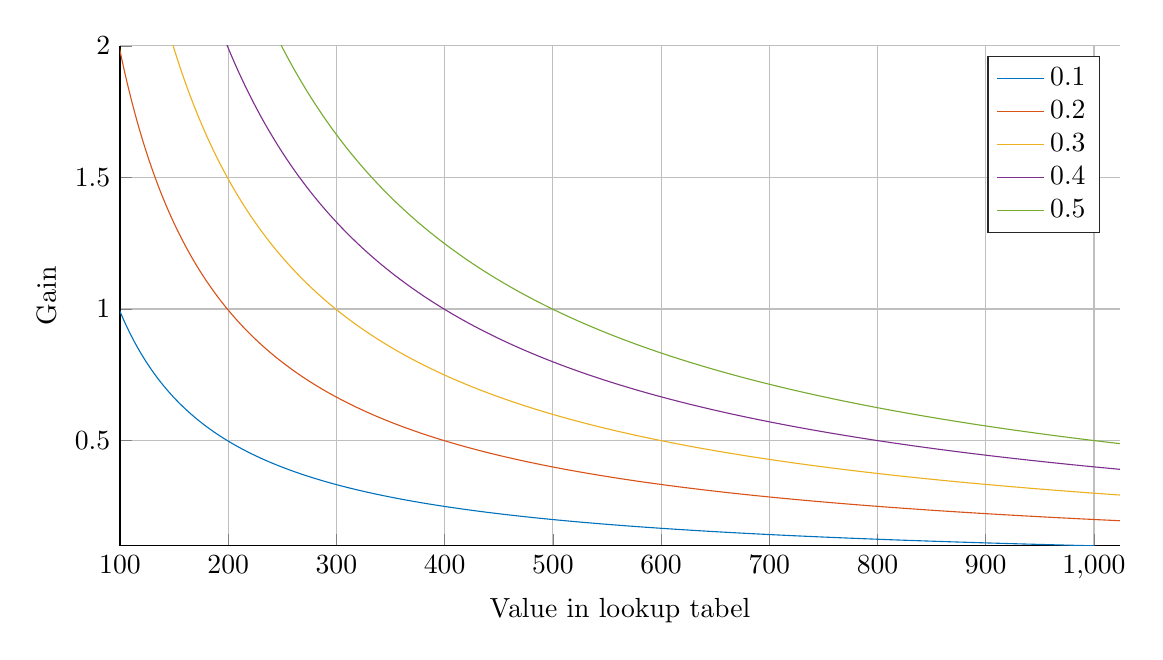
\begin{tikzpicture}

\begin{axis}[%
width=5in,
height=2.5in,
at={(0.758in,0.481in)},
scale only axis,
xmin=100,
xmax=1024,
xlabel={Value in lookup tabel},
xmajorgrids,
ymin=0.1,
ymax=2,
ylabel={Gain},
ymajorgrids,
axis background/.style={fill=white},
axis x line*=bottom,
axis y line*=left,
legend style={legend cell align=left,align=left,draw=white!15!black}
]
\addplot [color=mycolor1,solid]
  table[row sep=crcr]{%
99.0967741935484	1\\
100.097751710655	0.99009900990099\\
101.098729227761	0.980392156862745\\
102.099706744868	0.970873786407767\\
103.100684261975	0.961538461538462\\
104.101661779081	0.952380952380952\\
105.102639296188	0.943396226415094\\
106.103616813294	0.934579439252337\\
107.104594330401	0.925925925925926\\
108.105571847507	0.917431192660551\\
109.106549364614	0.909090909090909\\
110.10752688172	0.900900900900901\\
111.108504398827	0.892857142857143\\
112.109481915934	0.884955752212389\\
113.11045943304	0.87719298245614\\
114.111436950147	0.869565217391304\\
115.112414467253	0.862068965517241\\
116.11339198436	0.854700854700855\\
117.114369501466	0.847457627118644\\
118.115347018573	0.840336134453782\\
119.116324535679	0.833333333333333\\
120.117302052786	0.826446280991736\\
121.118279569892	0.819672131147541\\
122.119257086999	0.813008130081301\\
123.120234604106	0.806451612903226\\
124.121212121212	0.8\\
125.122189638319	0.793650793650794\\
126.123167155425	0.78740157480315\\
127.124144672532	0.78125\\
128.125122189638	0.775193798449612\\
129.126099706745	0.769230769230769\\
130.127077223851	0.763358778625954\\
131.128054740958	0.757575757575758\\
132.129032258065	0.75187969924812\\
133.130009775171	0.746268656716418\\
134.130987292278	0.740740740740741\\
135.131964809384	0.735294117647059\\
136.132942326491	0.72992700729927\\
137.133919843597	0.72463768115942\\
138.134897360704	0.719424460431655\\
139.13587487781	0.714285714285714\\
140.136852394917	0.709219858156029\\
141.137829912023	0.704225352112676\\
142.13880742913	0.699300699300699\\
143.139784946237	0.694444444444445\\
144.140762463343	0.689655172413793\\
145.14173998045	0.684931506849315\\
146.142717497556	0.680272108843538\\
147.143695014663	0.675675675675676\\
148.144672531769	0.671140939597315\\
149.145650048876	0.666666666666667\\
150.146627565982	0.662251655629139\\
151.147605083089	0.657894736842105\\
152.148582600196	0.65359477124183\\
153.149560117302	0.649350649350649\\
154.150537634409	0.645161290322581\\
155.151515151515	0.641025641025641\\
156.152492668622	0.636942675159236\\
157.153470185728	0.632911392405063\\
158.154447702835	0.628930817610063\\
159.155425219941	0.625\\
160.156402737048	0.62111801242236\\
161.157380254154	0.617283950617284\\
162.158357771261	0.613496932515337\\
163.159335288368	0.609756097560976\\
164.160312805474	0.606060606060606\\
165.161290322581	0.602409638554217\\
166.162267839687	0.598802395209581\\
167.163245356794	0.595238095238095\\
168.1642228739	0.591715976331361\\
169.165200391007	0.588235294117647\\
170.166177908113	0.584795321637427\\
171.16715542522	0.581395348837209\\
172.168132942326	0.578034682080925\\
173.169110459433	0.574712643678161\\
174.17008797654	0.571428571428572\\
175.171065493646	0.568181818181818\\
176.172043010753	0.564971751412429\\
177.173020527859	0.561797752808989\\
178.173998044966	0.558659217877095\\
179.174975562072	0.555555555555556\\
180.175953079179	0.552486187845304\\
181.176930596285	0.54945054945055\\
182.177908113392	0.546448087431694\\
183.178885630499	0.543478260869565\\
184.179863147605	0.540540540540541\\
185.180840664712	0.537634408602151\\
186.181818181818	0.53475935828877\\
187.182795698925	0.531914893617021\\
188.183773216031	0.529100529100529\\
189.184750733138	0.526315789473684\\
190.185728250244	0.523560209424084\\
191.186705767351	0.520833333333333\\
192.187683284457	0.518134715025907\\
193.188660801564	0.515463917525773\\
194.189638318671	0.512820512820513\\
195.190615835777	0.510204081632653\\
196.191593352884	0.50761421319797\\
197.19257086999	0.505050505050505\\
198.193548387097	0.50251256281407\\
199.194525904203	0.5\\
200.19550342131	0.497512437810945\\
201.196480938416	0.495049504950495\\
202.197458455523	0.492610837438424\\
203.19843597263	0.490196078431373\\
204.199413489736	0.487804878048781\\
205.200391006843	0.485436893203884\\
206.201368523949	0.483091787439614\\
207.202346041056	0.480769230769231\\
208.203323558162	0.478468899521531\\
209.204301075269	0.476190476190476\\
210.205278592375	0.4739336492891\\
211.206256109482	0.471698113207547\\
212.207233626588	0.469483568075117\\
213.208211143695	0.467289719626168\\
214.209188660802	0.465116279069767\\
215.210166177908	0.462962962962963\\
216.211143695015	0.460829493087558\\
217.212121212121	0.458715596330275\\
218.213098729228	0.45662100456621\\
219.214076246334	0.454545454545455\\
220.215053763441	0.452488687782805\\
221.216031280547	0.45045045045045\\
222.217008797654	0.448430493273543\\
223.217986314761	0.446428571428571\\
224.218963831867	0.444444444444444\\
225.219941348974	0.442477876106195\\
226.22091886608	0.440528634361234\\
227.221896383187	0.43859649122807\\
228.222873900293	0.436681222707424\\
229.2238514174	0.434782608695652\\
230.224828934506	0.432900432900433\\
231.225806451613	0.431034482758621\\
232.226783968719	0.429184549356223\\
233.227761485826	0.427350427350427\\
234.228739002933	0.425531914893617\\
235.229716520039	0.423728813559322\\
236.230694037146	0.421940928270042\\
237.231671554252	0.420168067226891\\
238.232649071359	0.418410041841004\\
239.233626588465	0.416666666666667\\
240.234604105572	0.4149377593361\\
241.235581622678	0.413223140495868\\
242.236559139785	0.411522633744856\\
243.237536656892	0.409836065573771\\
244.238514173998	0.408163265306122\\
245.239491691105	0.40650406504065\\
246.240469208211	0.404858299595142\\
247.241446725318	0.403225806451613\\
248.242424242424	0.401606425702811\\
249.243401759531	0.4\\
250.244379276637	0.398406374501992\\
251.245356793744	0.396825396825397\\
252.24633431085	0.395256916996047\\
253.247311827957	0.393700787401575\\
254.248289345064	0.392156862745098\\
255.24926686217	0.390625\\
256.250244379277	0.389105058365759\\
257.251221896383	0.387596899224806\\
258.25219941349	0.386100386100386\\
259.253176930596	0.384615384615385\\
260.254154447703	0.383141762452107\\
261.255131964809	0.381679389312977\\
262.256109481916	0.380228136882129\\
263.257086999022	0.378787878787879\\
264.258064516129	0.377358490566038\\
265.259042033236	0.37593984962406\\
266.260019550342	0.374531835205993\\
267.260997067449	0.373134328358209\\
268.261974584555	0.371747211895911\\
269.262952101662	0.37037037037037\\
270.263929618768	0.3690036900369\\
271.264907135875	0.367647058823529\\
272.265884652981	0.366300366300366\\
273.266862170088	0.364963503649635\\
274.267839687195	0.363636363636364\\
275.268817204301	0.36231884057971\\
276.269794721408	0.36101083032491\\
277.270772238514	0.359712230215827\\
278.271749755621	0.3584229390681\\
279.272727272727	0.357142857142857\\
280.273704789834	0.355871886120996\\
281.27468230694	0.354609929078014\\
282.275659824047	0.353356890459364\\
283.276637341153	0.352112676056338\\
284.27761485826	0.350877192982456\\
285.278592375367	0.34965034965035\\
286.279569892473	0.348432055749129\\
287.28054740958	0.347222222222222\\
288.281524926686	0.346020761245675\\
289.282502443793	0.344827586206897\\
290.283479960899	0.343642611683849\\
291.284457478006	0.342465753424658\\
292.285434995112	0.341296928327645\\
293.286412512219	0.340136054421769\\
294.287390029326	0.338983050847458\\
295.288367546432	0.337837837837838\\
296.289345063539	0.336700336700337\\
297.290322580645	0.335570469798658\\
298.291300097752	0.334448160535117\\
299.292277614858	0.333333333333333\\
300.293255131965	0.332225913621262\\
301.294232649071	0.33112582781457\\
302.295210166178	0.33003300330033\\
303.296187683284	0.328947368421053\\
304.297165200391	0.327868852459016\\
305.298142717498	0.326797385620915\\
306.299120234604	0.325732899022801\\
307.300097751711	0.324675324675325\\
308.301075268817	0.323624595469256\\
309.302052785924	0.32258064516129\\
310.30303030303	0.321543408360129\\
311.304007820137	0.320512820512821\\
312.304985337243	0.319488817891374\\
313.30596285435	0.318471337579618\\
314.306940371457	0.317460317460318\\
315.307917888563	0.316455696202532\\
316.30889540567	0.315457413249211\\
317.309872922776	0.314465408805031\\
318.310850439883	0.313479623824451\\
319.311827956989	0.3125\\
320.312805474096	0.311526479750779\\
321.313782991202	0.31055900621118\\
322.314760508309	0.309597523219814\\
323.315738025415	0.308641975308642\\
324.316715542522	0.307692307692308\\
325.317693059629	0.306748466257669\\
326.318670576735	0.305810397553517\\
327.319648093842	0.304878048780488\\
328.320625610948	0.303951367781155\\
329.321603128055	0.303030303030303\\
330.322580645161	0.302114803625378\\
331.323558162268	0.301204819277108\\
332.324535679374	0.3003003003003\\
333.325513196481	0.29940119760479\\
334.326490713587	0.298507462686567\\
335.327468230694	0.297619047619048\\
336.328445747801	0.29673590504451\\
337.329423264907	0.29585798816568\\
338.330400782014	0.294985250737463\\
339.33137829912	0.294117647058824\\
340.332355816227	0.293255131964809\\
341.333333333333	0.292397660818713\\
342.33431085044	0.291545189504373\\
343.335288367546	0.290697674418605\\
344.336265884653	0.289855072463768\\
345.33724340176	0.289017341040462\\
346.338220918866	0.288184438040346\\
347.339198435973	0.287356321839081\\
348.340175953079	0.286532951289398\\
349.341153470186	0.285714285714286\\
350.342130987292	0.284900284900285\\
351.343108504399	0.284090909090909\\
352.344086021505	0.28328611898017\\
353.345063538612	0.282485875706215\\
354.346041055719	0.28169014084507\\
355.347018572825	0.280898876404494\\
356.347996089932	0.280112044817927\\
357.348973607038	0.279329608938548\\
358.349951124145	0.278551532033426\\
359.350928641251	0.277777777777778\\
360.351906158358	0.277008310249308\\
361.352883675464	0.276243093922652\\
362.353861192571	0.275482093663912\\
363.354838709677	0.274725274725275\\
364.355816226784	0.273972602739726\\
365.356793743891	0.273224043715847\\
366.357771260997	0.272479564032698\\
367.358748778104	0.271739130434783\\
368.35972629521	0.2710027100271\\
369.360703812317	0.27027027027027\\
370.361681329423	0.269541778975741\\
371.36265884653	0.268817204301075\\
372.363636363636	0.268096514745308\\
373.364613880743	0.267379679144385\\
374.365591397849	0.266666666666667\\
375.366568914956	0.265957446808511\\
376.367546432063	0.26525198938992\\
377.368523949169	0.264550264550265\\
378.369501466276	0.263852242744063\\
379.370478983382	0.263157894736842\\
380.371456500489	0.26246719160105\\
381.372434017595	0.261780104712042\\
382.373411534702	0.261096605744125\\
383.374389051808	0.260416666666667\\
384.375366568915	0.25974025974026\\
385.376344086022	0.259067357512953\\
386.377321603128	0.258397932816538\\
387.378299120235	0.257731958762887\\
388.379276637341	0.25706940874036\\
389.380254154448	0.256410256410256\\
390.381231671554	0.255754475703325\\
391.382209188661	0.255102040816327\\
392.383186705767	0.254452926208651\\
393.384164222874	0.253807106598985\\
394.38514173998	0.253164556962025\\
395.386119257087	0.252525252525253\\
396.387096774194	0.251889168765743\\
397.3880742913	0.251256281407035\\
398.389051808407	0.25062656641604\\
399.390029325513	0.25\\
400.39100684262	0.249376558603491\\
401.391984359726	0.248756218905473\\
402.392961876833	0.248138957816377\\
403.393939393939	0.247524752475248\\
404.394916911046	0.246913580246914\\
405.395894428152	0.246305418719212\\
406.396871945259	0.245700245700246\\
407.397849462366	0.245098039215686\\
408.398826979472	0.244498777506112\\
409.399804496579	0.24390243902439\\
410.400782013685	0.24330900243309\\
411.401759530792	0.242718446601942\\
412.402737047898	0.242130750605327\\
413.403714565005	0.241545893719807\\
414.404692082111	0.240963855421687\\
415.405669599218	0.240384615384615\\
416.406647116325	0.239808153477218\\
417.407624633431	0.239234449760766\\
418.408602150538	0.238663484486874\\
419.409579667644	0.238095238095238\\
420.410557184751	0.237529691211401\\
421.411534701857	0.23696682464455\\
422.412512218964	0.236406619385343\\
423.41348973607	0.235849056603774\\
424.414467253177	0.235294117647059\\
425.415444770284	0.234741784037559\\
426.41642228739	0.234192037470726\\
427.417399804497	0.233644859813084\\
428.418377321603	0.233100233100233\\
429.41935483871	0.232558139534884\\
430.420332355816	0.232018561484919\\
431.421309872923	0.231481481481482\\
432.422287390029	0.23094688221709\\
433.423264907136	0.230414746543779\\
434.424242424242	0.229885057471264\\
435.425219941349	0.229357798165138\\
436.426197458456	0.22883295194508\\
437.427174975562	0.228310502283105\\
438.428152492669	0.227790432801822\\
439.429130009775	0.227272727272727\\
440.430107526882	0.226757369614512\\
441.431085043988	0.226244343891403\\
442.432062561095	0.225733634311512\\
443.433040078201	0.225225225225225\\
444.434017595308	0.224719101123596\\
445.434995112414	0.224215246636771\\
446.435972629521	0.223713646532439\\
447.436950146628	0.223214285714286\\
448.437927663734	0.22271714922049\\
449.438905180841	0.222222222222222\\
450.439882697947	0.221729490022173\\
451.440860215054	0.221238938053097\\
452.44183773216	0.22075055187638\\
453.442815249267	0.220264317180617\\
454.443792766373	0.21978021978022\\
455.44477028348	0.219298245614035\\
456.445747800587	0.218818380743982\\
457.446725317693	0.218340611353712\\
458.4477028348	0.217864923747277\\
459.448680351906	0.217391304347826\\
460.449657869013	0.216919739696312\\
461.450635386119	0.216450216450216\\
462.451612903226	0.215982721382289\\
463.452590420332	0.21551724137931\\
464.453567937439	0.21505376344086\\
465.454545454545	0.214592274678112\\
466.455522971652	0.214132762312634\\
467.456500488759	0.213675213675214\\
468.457478005865	0.213219616204691\\
469.458455522972	0.212765957446809\\
470.459433040078	0.212314225053079\\
471.460410557185	0.211864406779661\\
472.461388074291	0.211416490486258\\
473.462365591398	0.210970464135021\\
474.463343108504	0.210526315789474\\
475.464320625611	0.210084033613445\\
476.465298142717	0.209643605870021\\
477.466275659824	0.209205020920502\\
478.467253176931	0.208768267223382\\
479.468230694037	0.208333333333333\\
480.469208211144	0.207900207900208\\
481.47018572825	0.20746887966805\\
482.471163245357	0.20703933747412\\
483.472140762463	0.206611570247934\\
484.47311827957	0.206185567010309\\
485.474095796676	0.205761316872428\\
486.475073313783	0.205338809034908\\
487.47605083089	0.204918032786885\\
488.477028347996	0.204498977505112\\
489.478005865103	0.204081632653061\\
490.478983382209	0.203665987780041\\
491.479960899316	0.203252032520325\\
492.480938416422	0.202839756592292\\
493.481915933529	0.202429149797571\\
494.482893450635	0.202020202020202\\
495.483870967742	0.201612903225806\\
496.484848484849	0.201207243460765\\
497.485826001955	0.200803212851406\\
498.486803519062	0.200400801603206\\
499.487781036168	0.2\\
500.488758553275	0.199600798403194\\
501.489736070381	0.199203187250996\\
502.490713587488	0.198807157057654\\
503.491691104594	0.198412698412698\\
504.492668621701	0.198019801980198\\
505.493646138807	0.197628458498024\\
506.494623655914	0.19723865877712\\
507.495601173021	0.196850393700787\\
508.496578690127	0.196463654223969\\
509.497556207234	0.196078431372549\\
510.49853372434	0.195694716242661\\
511.499511241447	0.1953125\\
512.500488758553	0.194931773879142\\
513.50146627566	0.194552529182879\\
514.502443792766	0.194174757281553\\
515.503421309873	0.193798449612403\\
516.504398826979	0.193423597678917\\
517.505376344086	0.193050193050193\\
518.506353861193	0.192678227360308\\
519.507331378299	0.192307692307692\\
520.508308895406	0.191938579654511\\
521.509286412512	0.191570881226054\\
522.510263929619	0.191204588910134\\
523.511241446725	0.190839694656489\\
524.512218963832	0.19047619047619\\
525.513196480938	0.190114068441065\\
526.514173998045	0.189753320683112\\
527.515151515152	0.189393939393939\\
528.516129032258	0.189035916824197\\
529.517106549365	0.188679245283019\\
530.518084066471	0.188323917137476\\
531.519061583578	0.18796992481203\\
532.520039100684	0.187617260787992\\
533.521016617791	0.187265917602996\\
534.521994134897	0.186915887850467\\
535.522971652004	0.186567164179104\\
536.52394916911	0.186219739292365\\
537.524926686217	0.185873605947955\\
538.525904203324	0.185528756957328\\
539.52688172043	0.185185185185185\\
540.527859237537	0.184842883548983\\
541.528836754643	0.18450184501845\\
542.52981427175	0.184162062615101\\
543.530791788856	0.183823529411765\\
544.531769305963	0.18348623853211\\
545.532746823069	0.183150183150183\\
546.533724340176	0.182815356489945\\
547.534701857282	0.182481751824818\\
548.535679374389	0.182149362477231\\
549.536656891496	0.181818181818182\\
550.537634408602	0.181488203266788\\
551.538611925709	0.181159420289855\\
552.539589442815	0.180831826401447\\
553.540566959922	0.180505415162455\\
554.541544477028	0.18018018018018\\
555.542521994135	0.179856115107914\\
556.543499511241	0.179533213644524\\
557.544477028348	0.17921146953405\\
558.545454545455	0.178890876565295\\
559.546432062561	0.178571428571429\\
560.547409579668	0.17825311942959\\
561.548387096774	0.177935943060498\\
562.549364613881	0.177619893428064\\
563.550342130987	0.177304964539007\\
564.551319648094	0.176991150442478\\
565.5522971652	0.176678445229682\\
566.553274682307	0.17636684303351\\
567.554252199413	0.176056338028169\\
568.55522971652	0.175746924428823\\
569.556207233627	0.175438596491228\\
570.557184750733	0.175131348511384\\
571.55816226784	0.174825174825175\\
572.559139784946	0.174520069808028\\
573.560117302053	0.174216027874564\\
574.561094819159	0.173913043478261\\
575.562072336266	0.173611111111111\\
576.563049853372	0.173310225303293\\
577.564027370479	0.173010380622837\\
578.565004887586	0.172711571675302\\
579.565982404692	0.172413793103448\\
580.566959921799	0.172117039586919\\
581.567937438905	0.171821305841924\\
582.568914956012	0.171526586620926\\
583.569892473118	0.171232876712329\\
584.570869990225	0.170940170940171\\
585.571847507331	0.170648464163823\\
586.572825024438	0.170357751277683\\
587.573802541545	0.170068027210884\\
588.574780058651	0.169779286926995\\
589.575757575758	0.169491525423729\\
590.576735092864	0.169204737732657\\
591.577712609971	0.168918918918919\\
592.578690127077	0.168634064080944\\
593.579667644184	0.168350168350168\\
594.58064516129	0.168067226890756\\
595.581622678397	0.167785234899329\\
596.582600195503	0.16750418760469\\
597.58357771261	0.167224080267559\\
598.584555229717	0.166944908180301\\
599.585532746823	0.166666666666667\\
600.58651026393	0.166389351081531\\
601.587487781036	0.166112956810631\\
602.588465298143	0.165837479270315\\
603.589442815249	0.165562913907285\\
604.590420332356	0.165289256198347\\
605.591397849462	0.165016501650165\\
606.592375366569	0.164744645799012\\
607.593352883675	0.164473684210526\\
608.594330400782	0.164203612479475\\
609.595307917889	0.163934426229508\\
610.596285434995	0.16366612111293\\
611.597262952102	0.163398692810458\\
612.598240469208	0.163132137030995\\
613.599217986315	0.162866449511401\\
614.600195503421	0.16260162601626\\
615.601173020528	0.162337662337662\\
616.602150537634	0.162074554294976\\
617.603128054741	0.161812297734628\\
618.604105571848	0.161550888529887\\
619.605083088954	0.161290322580645\\
620.606060606061	0.161030595813205\\
621.607038123167	0.160771704180064\\
622.608015640274	0.160513643659711\\
623.60899315738	0.16025641025641\\
624.609970674487	0.16\\
625.610948191593	0.159744408945687\\
626.6119257087	0.159489633173844\\
627.612903225806	0.159235668789809\\
628.613880742913	0.158982511923688\\
629.61485826002	0.158730158730159\\
630.615835777126	0.158478605388273\\
631.616813294233	0.158227848101266\\
632.617790811339	0.157977883096367\\
633.618768328446	0.157728706624606\\
634.619745845552	0.15748031496063\\
635.620723362659	0.157232704402516\\
636.621700879765	0.156985871271586\\
637.622678396872	0.156739811912226\\
638.623655913979	0.156494522691706\\
639.624633431085	0.15625\\
640.625610948192	0.15600624024961\\
641.626588465298	0.155763239875389\\
642.627565982405	0.15552099533437\\
643.628543499511	0.15527950310559\\
644.629521016618	0.155038759689922\\
645.630498533724	0.154798761609907\\
646.631476050831	0.154559505409583\\
647.632453567937	0.154320987654321\\
648.633431085044	0.154083204930663\\
649.634408602151	0.153846153846154\\
650.635386119257	0.153609831029186\\
651.636363636364	0.153374233128834\\
652.63734115347	0.153139356814701\\
653.638318670577	0.152905198776758\\
654.639296187683	0.152671755725191\\
655.64027370479	0.152439024390244\\
656.641251221896	0.15220700152207\\
657.642228739003	0.151975683890578\\
658.643206256109	0.151745068285281\\
659.644183773216	0.151515151515152\\
660.645161290323	0.151285930408472\\
661.646138807429	0.151057401812689\\
662.647116324536	0.150829562594268\\
663.648093841642	0.150602409638554\\
664.649071358749	0.150375939849624\\
665.650048875855	0.15015015015015\\
666.651026392962	0.149925037481259\\
667.652003910068	0.149700598802395\\
668.652981427175	0.149476831091181\\
669.653958944282	0.149253731343284\\
670.654936461388	0.14903129657228\\
671.655913978495	0.148809523809524\\
672.656891495601	0.148588410104012\\
673.657869012708	0.148367952522255\\
674.658846529814	0.148148148148148\\
675.659824046921	0.14792899408284\\
676.660801564027	0.147710487444609\\
677.661779081134	0.147492625368732\\
678.66275659824	0.147275405007364\\
679.663734115347	0.147058823529412\\
680.664711632454	0.146842878120411\\
681.66568914956	0.146627565982405\\
682.666666666667	0.146412884333821\\
683.667644183773	0.146198830409357\\
684.66862170088	0.145985401459854\\
685.669599217986	0.145772594752187\\
686.670576735093	0.145560407569141\\
687.671554252199	0.145348837209302\\
688.672531769306	0.145137880986938\\
689.673509286412	0.144927536231884\\
690.674486803519	0.144717800289436\\
691.675464320626	0.144508670520231\\
692.676441837732	0.144300144300144\\
693.677419354839	0.144092219020173\\
694.678396871945	0.143884892086331\\
695.679374389052	0.14367816091954\\
696.680351906158	0.143472022955524\\
697.681329423265	0.143266475644699\\
698.682306940371	0.143061516452074\\
699.683284457478	0.142857142857143\\
700.684261974585	0.14265335235378\\
701.685239491691	0.142450142450142\\
702.686217008798	0.142247510668563\\
703.687194525904	0.142045454545455\\
704.688172043011	0.141843971631206\\
705.689149560117	0.141643059490085\\
706.690127077224	0.141442715700141\\
707.69110459433	0.141242937853107\\
708.692082111437	0.141043723554302\\
709.693059628544	0.140845070422535\\
710.69403714565	0.140646976090014\\
711.695014662757	0.140449438202247\\
712.695992179863	0.140252454417952\\
713.69696969697	0.140056022408964\\
714.697947214076	0.13986013986014\\
715.698924731183	0.139664804469274\\
716.699902248289	0.139470013947001\\
717.700879765396	0.139275766016713\\
718.701857282502	0.139082058414465\\
719.702834799609	0.138888888888889\\
720.703812316716	0.13869625520111\\
721.704789833822	0.138504155124654\\
722.705767350929	0.138312586445367\\
723.706744868035	0.138121546961326\\
724.707722385142	0.137931034482759\\
725.708699902248	0.137741046831956\\
726.709677419355	0.137551581843191\\
727.710654936461	0.137362637362637\\
728.711632453568	0.137174211248285\\
729.712609970675	0.136986301369863\\
730.713587487781	0.136798905608755\\
731.714565004888	0.136612021857924\\
732.715542521994	0.136425648021828\\
733.716520039101	0.136239782016349\\
734.717497556207	0.136054421768708\\
735.718475073314	0.135869565217391\\
736.71945259042	0.135685210312076\\
737.720430107527	0.13550135501355\\
738.721407624633	0.13531799729364\\
739.72238514174	0.135135135135135\\
740.723362658847	0.134952766531714\\
741.724340175953	0.134770889487871\\
742.72531769306	0.134589502018843\\
743.726295210166	0.134408602150538\\
744.727272727273	0.134228187919463\\
745.728250244379	0.134048257372654\\
746.729227761486	0.133868808567604\\
747.730205278592	0.133689839572193\\
748.731182795699	0.13351134846462\\
749.732160312805	0.133333333333333\\
750.733137829912	0.133155792276964\\
751.734115347019	0.132978723404255\\
752.735092864125	0.132802124833997\\
753.736070381232	0.13262599469496\\
754.737047898338	0.132450331125828\\
755.738025415445	0.132275132275132\\
756.739002932551	0.132100396301189\\
757.739980449658	0.131926121372032\\
758.740957966764	0.131752305665349\\
759.741935483871	0.131578947368421\\
760.742913000978	0.131406044678055\\
761.743890518084	0.131233595800525\\
762.744868035191	0.131061598951507\\
763.745845552297	0.130890052356021\\
764.746823069404	0.130718954248366\\
765.74780058651	0.130548302872063\\
766.748778103617	0.130378096479791\\
767.749755620723	0.130208333333333\\
768.75073313783	0.130039011703511\\
769.751710654936	0.12987012987013\\
770.752688172043	0.12970168612192\\
771.75366568915	0.129533678756477\\
772.754643206256	0.129366106080207\\
773.755620723363	0.129198966408269\\
774.756598240469	0.129032258064516\\
775.757575757576	0.128865979381443\\
776.758553274682	0.128700128700129\\
777.759530791789	0.12853470437018\\
778.760508308895	0.128369704749679\\
779.761485826002	0.128205128205128\\
780.762463343108	0.128040973111396\\
781.763440860215	0.127877237851662\\
782.764418377322	0.127713920817369\\
783.765395894428	0.127551020408163\\
784.766373411535	0.127388535031847\\
785.767350928641	0.127226463104326\\
786.768328445748	0.127064803049555\\
787.769305962854	0.126903553299492\\
788.770283479961	0.126742712294043\\
789.771260997067	0.126582278481013\\
790.772238514174	0.126422250316056\\
791.773216031281	0.126262626262626\\
792.774193548387	0.126103404791929\\
793.775171065494	0.125944584382872\\
794.7761485826	0.125786163522013\\
795.777126099707	0.125628140703518\\
796.778103616813	0.125470514429109\\
797.77908113392	0.12531328320802\\
798.780058651026	0.125156445556946\\
799.781036168133	0.125\\
800.782013685239	0.124843945068664\\
801.782991202346	0.124688279301746\\
802.783968719453	0.12453300124533\\
803.784946236559	0.124378109452736\\
804.785923753666	0.124223602484472\\
805.786901270772	0.124069478908189\\
806.787878787879	0.123915737298637\\
807.788856304985	0.123762376237624\\
808.789833822092	0.123609394313968\\
809.790811339198	0.123456790123457\\
810.791788856305	0.123304562268804\\
811.792766373412	0.123152709359606\\
812.793743890518	0.1230012300123\\
813.794721407625	0.122850122850123\\
814.795698924731	0.122699386503068\\
815.796676441838	0.122549019607843\\
816.797653958944	0.122399020807834\\
817.798631476051	0.122249388753056\\
818.799608993157	0.122100122100122\\
819.800586510264	0.121951219512195\\
820.80156402737	0.121802679658953\\
821.802541544477	0.121654501216545\\
822.803519061584	0.121506682867558\\
823.80449657869	0.121359223300971\\
824.805474095797	0.121212121212121\\
825.806451612903	0.121065375302663\\
826.80742913001	0.120918984280532\\
827.808406647116	0.120772946859903\\
828.809384164223	0.120627261761158\\
829.810361681329	0.120481927710843\\
830.811339198436	0.120336943441637\\
831.812316715542	0.120192307692308\\
832.813294232649	0.120048019207683\\
833.814271749756	0.119904076738609\\
834.815249266862	0.119760479041916\\
835.816226783969	0.119617224880383\\
836.817204301075	0.1194743130227\\
837.818181818182	0.119331742243437\\
838.819159335288	0.119189511323004\\
839.820136852395	0.119047619047619\\
840.821114369502	0.118906064209275\\
841.822091886608	0.118764845605701\\
842.823069403715	0.118623962040332\\
843.824046920821	0.118483412322275\\
844.825024437928	0.118343195266272\\
845.826001955034	0.118203309692671\\
846.826979472141	0.118063754427391\\
847.827956989247	0.117924528301887\\
848.828934506354	0.117785630153121\\
849.82991202346	0.117647058823529\\
850.830889540567	0.117508813160987\\
851.831867057674	0.117370892018779\\
852.83284457478	0.117233294255569\\
853.833822091887	0.117096018735363\\
854.834799608993	0.116959064327485\\
855.8357771261	0.116822429906542\\
856.836754643206	0.116686114352392\\
857.837732160313	0.116550116550117\\
858.838709677419	0.116414435389988\\
859.839687194526	0.116279069767442\\
860.840664711632	0.116144018583043\\
861.841642228739	0.116009280742459\\
862.842619745846	0.115874855156431\\
863.843597262952	0.115740740740741\\
864.844574780059	0.115606936416185\\
865.845552297165	0.115473441108545\\
866.846529814272	0.115340253748558\\
867.847507331378	0.115207373271889\\
868.848484848485	0.115074798619102\\
869.849462365591	0.114942528735632\\
870.850439882698	0.114810562571757\\
871.851417399805	0.114678899082569\\
872.852394916911	0.11454753722795\\
873.853372434018	0.11441647597254\\
874.854349951124	0.114285714285714\\
875.855327468231	0.114155251141553\\
876.856304985337	0.114025085518814\\
877.857282502444	0.113895216400911\\
878.85826001955	0.113765642775882\\
879.859237536657	0.113636363636364\\
880.860215053763	0.113507377979569\\
881.86119257087	0.113378684807256\\
882.862170087977	0.113250283125708\\
883.863147605083	0.113122171945701\\
884.86412512219	0.112994350282486\\
885.865102639296	0.112866817155756\\
886.866080156403	0.112739571589628\\
887.867057673509	0.112612612612613\\
888.868035190616	0.112485939257593\\
889.869012707722	0.112359550561798\\
890.869990224829	0.112233445566779\\
891.870967741935	0.112107623318386\\
892.871945259042	0.111982082866741\\
893.872922776149	0.111856823266219\\
894.873900293255	0.111731843575419\\
895.874877810362	0.111607142857143\\
896.875855327468	0.111482720178372\\
897.876832844575	0.111358574610245\\
898.877810361681	0.111234705228031\\
899.878787878788	0.111111111111111\\
900.879765395894	0.110987791342952\\
901.880742913001	0.110864745011086\\
902.881720430108	0.110741971207087\\
903.882697947214	0.110619469026549\\
904.883675464321	0.110497237569061\\
905.884652981427	0.11037527593819\\
906.885630498534	0.110253583241455\\
907.88660801564	0.110132158590308\\
908.887585532747	0.11001100110011\\
909.888563049853	0.10989010989011\\
910.88954056696	0.109769484083425\\
911.890518084066	0.109649122807018\\
912.891495601173	0.109529025191676\\
913.89247311828	0.109409190371991\\
914.893450635386	0.109289617486339\\
915.894428152493	0.109170305676856\\
916.895405669599	0.109051254089422\\
917.896383186706	0.108932461873638\\
918.897360703812	0.108813928182807\\
919.898338220919	0.108695652173913\\
920.899315738025	0.1085776330076\\
921.900293255132	0.108459869848156\\
922.901270772238	0.108342361863489\\
923.902248289345	0.108225108225108\\
924.903225806452	0.108108108108108\\
925.904203323558	0.107991360691145\\
926.905180840665	0.107874865156419\\
927.906158357771	0.107758620689655\\
928.907135874878	0.107642626480086\\
929.908113391984	0.10752688172043\\
930.909090909091	0.107411385606874\\
931.910068426197	0.107296137339056\\
932.911045943304	0.107181136120043\\
933.912023460411	0.107066381156317\\
934.913000977517	0.106951871657754\\
935.913978494624	0.106837606837607\\
936.91495601173	0.106723585912487\\
937.915933528837	0.106609808102345\\
938.916911045943	0.106496272630458\\
939.91788856305	0.106382978723404\\
940.918866080156	0.106269925611052\\
941.919843597263	0.106157112526539\\
942.920821114369	0.106044538706257\\
943.921798631476	0.105932203389831\\
944.922776148583	0.105820105820106\\
945.923753665689	0.105708245243129\\
946.924731182796	0.105596620908131\\
947.925708699902	0.105485232067511\\
948.926686217009	0.105374077976818\\
949.927663734115	0.105263157894737\\
950.928641251222	0.10515247108307\\
951.929618768328	0.105042016806723\\
952.930596285435	0.104931794333683\\
953.931573802541	0.10482180293501\\
954.932551319648	0.104712041884817\\
955.933528836755	0.104602510460251\\
956.934506353861	0.104493207941484\\
957.935483870968	0.104384133611691\\
958.936461388074	0.104275286757039\\
959.937438905181	0.104166666666667\\
960.938416422287	0.104058272632674\\
961.939393939394	0.103950103950104\\
962.940371456501	0.103842159916926\\
963.941348973607	0.103734439834025\\
964.942326490714	0.103626943005181\\
965.94330400782	0.10351966873706\\
966.944281524927	0.103412616339193\\
967.945259042033	0.103305785123967\\
968.94623655914	0.103199174406605\\
969.947214076246	0.103092783505155\\
970.948191593353	0.102986611740474\\
971.949169110459	0.102880658436214\\
972.950146627566	0.102774922918808\\
973.951124144673	0.102669404517454\\
974.952101661779	0.102564102564103\\
975.953079178886	0.102459016393443\\
976.954056695992	0.102354145342886\\
977.955034213099	0.102249488752556\\
978.956011730205	0.102145045965271\\
979.956989247312	0.102040816326531\\
980.957966764418	0.101936799184506\\
981.958944281525	0.10183299389002\\
982.959921798632	0.101729399796541\\
983.960899315738	0.101626016260163\\
984.961876832845	0.101522842639594\\
985.962854349951	0.101419878296146\\
986.963831867058	0.101317122593718\\
987.964809384164	0.101214574898785\\
988.965786901271	0.101112234580384\\
989.966764418377	0.101010101010101\\
990.967741935484	0.100908173562059\\
991.96871945259	0.100806451612903\\
992.969696969697	0.100704934541793\\
993.970674486804	0.100603621730382\\
994.97165200391	0.100502512562814\\
995.972629521017	0.100401606425703\\
996.973607038123	0.100300902708124\\
997.97458455523	0.100200400801603\\
998.975562072336	0.1001001001001\\
999.976539589443	0.1\\
1000.97751710655	0.0999000999000999\\
};
\addlegendentry{0.1};

\addplot [color=mycolor2,solid]
  table[row sep=crcr]{%
99.0967741935484	2\\
100.097751710655	1.98019801980198\\
101.098729227761	1.96078431372549\\
102.099706744868	1.94174757281553\\
103.100684261975	1.92307692307692\\
104.101661779081	1.9047619047619\\
105.102639296188	1.88679245283019\\
106.103616813294	1.86915887850467\\
107.104594330401	1.85185185185185\\
108.105571847507	1.8348623853211\\
109.106549364614	1.81818181818182\\
110.10752688172	1.8018018018018\\
111.108504398827	1.78571428571429\\
112.109481915934	1.76991150442478\\
113.11045943304	1.75438596491228\\
114.111436950147	1.73913043478261\\
115.112414467253	1.72413793103448\\
116.11339198436	1.70940170940171\\
117.114369501466	1.69491525423729\\
118.115347018573	1.68067226890756\\
119.116324535679	1.66666666666667\\
120.117302052786	1.65289256198347\\
121.118279569892	1.63934426229508\\
122.119257086999	1.6260162601626\\
123.120234604106	1.61290322580645\\
124.121212121212	1.6\\
125.122189638319	1.58730158730159\\
126.123167155425	1.5748031496063\\
127.124144672532	1.5625\\
128.125122189638	1.55038759689922\\
129.126099706745	1.53846153846154\\
130.127077223851	1.52671755725191\\
131.128054740958	1.51515151515152\\
132.129032258065	1.50375939849624\\
133.130009775171	1.49253731343284\\
134.130987292278	1.48148148148148\\
135.131964809384	1.47058823529412\\
136.132942326491	1.45985401459854\\
137.133919843597	1.44927536231884\\
138.134897360704	1.43884892086331\\
139.13587487781	1.42857142857143\\
140.136852394917	1.41843971631206\\
141.137829912023	1.40845070422535\\
142.13880742913	1.3986013986014\\
143.139784946237	1.38888888888889\\
144.140762463343	1.37931034482759\\
145.14173998045	1.36986301369863\\
146.142717497556	1.36054421768708\\
147.143695014663	1.35135135135135\\
148.144672531769	1.34228187919463\\
149.145650048876	1.33333333333333\\
150.146627565982	1.32450331125828\\
151.147605083089	1.31578947368421\\
152.148582600196	1.30718954248366\\
153.149560117302	1.2987012987013\\
154.150537634409	1.29032258064516\\
155.151515151515	1.28205128205128\\
156.152492668622	1.27388535031847\\
157.153470185728	1.26582278481013\\
158.154447702835	1.25786163522013\\
159.155425219941	1.25\\
160.156402737048	1.24223602484472\\
161.157380254154	1.23456790123457\\
162.158357771261	1.22699386503067\\
163.159335288368	1.21951219512195\\
164.160312805474	1.21212121212121\\
165.161290322581	1.20481927710843\\
166.162267839687	1.19760479041916\\
167.163245356794	1.19047619047619\\
168.1642228739	1.18343195266272\\
169.165200391007	1.17647058823529\\
170.166177908113	1.16959064327485\\
171.16715542522	1.16279069767442\\
172.168132942326	1.15606936416185\\
173.169110459433	1.14942528735632\\
174.17008797654	1.14285714285714\\
175.171065493646	1.13636363636364\\
176.172043010753	1.12994350282486\\
177.173020527859	1.12359550561798\\
178.173998044966	1.11731843575419\\
179.174975562072	1.11111111111111\\
180.175953079179	1.10497237569061\\
181.176930596285	1.0989010989011\\
182.177908113392	1.09289617486339\\
183.178885630499	1.08695652173913\\
184.179863147605	1.08108108108108\\
185.180840664712	1.0752688172043\\
186.181818181818	1.06951871657754\\
187.182795698925	1.06382978723404\\
188.183773216031	1.05820105820106\\
189.184750733138	1.05263157894737\\
190.185728250244	1.04712041884817\\
191.186705767351	1.04166666666667\\
192.187683284457	1.03626943005181\\
193.188660801564	1.03092783505155\\
194.189638318671	1.02564102564103\\
195.190615835777	1.02040816326531\\
196.191593352884	1.01522842639594\\
197.19257086999	1.01010101010101\\
198.193548387097	1.00502512562814\\
199.194525904203	1\\
200.19550342131	0.995024875621891\\
201.196480938416	0.99009900990099\\
202.197458455523	0.985221674876847\\
203.19843597263	0.980392156862745\\
204.199413489736	0.975609756097561\\
205.200391006843	0.970873786407767\\
206.201368523949	0.966183574879227\\
207.202346041056	0.961538461538462\\
208.203323558162	0.956937799043062\\
209.204301075269	0.952380952380952\\
210.205278592375	0.947867298578199\\
211.206256109482	0.943396226415094\\
212.207233626588	0.938967136150235\\
213.208211143695	0.934579439252337\\
214.209188660802	0.930232558139535\\
215.210166177908	0.925925925925926\\
216.211143695015	0.921658986175115\\
217.212121212121	0.917431192660551\\
218.213098729228	0.91324200913242\\
219.214076246334	0.909090909090909\\
220.215053763441	0.904977375565611\\
221.216031280547	0.900900900900901\\
222.217008797654	0.896860986547085\\
223.217986314761	0.892857142857143\\
224.218963831867	0.888888888888889\\
225.219941348974	0.884955752212389\\
226.22091886608	0.881057268722467\\
227.221896383187	0.87719298245614\\
228.222873900293	0.873362445414847\\
229.2238514174	0.869565217391304\\
230.224828934506	0.865800865800866\\
231.225806451613	0.862068965517241\\
232.226783968719	0.858369098712446\\
233.227761485826	0.854700854700855\\
234.228739002933	0.851063829787234\\
235.229716520039	0.847457627118644\\
236.230694037146	0.843881856540085\\
237.231671554252	0.840336134453782\\
238.232649071359	0.836820083682008\\
239.233626588465	0.833333333333333\\
240.234604105572	0.829875518672199\\
241.235581622678	0.826446280991736\\
242.236559139785	0.823045267489712\\
243.237536656892	0.819672131147541\\
244.238514173998	0.816326530612245\\
245.239491691105	0.813008130081301\\
246.240469208211	0.809716599190283\\
247.241446725318	0.806451612903226\\
248.242424242424	0.803212851405622\\
249.243401759531	0.8\\
250.244379276637	0.796812749003984\\
251.245356793744	0.793650793650794\\
252.24633431085	0.790513833992095\\
253.247311827957	0.78740157480315\\
254.248289345064	0.784313725490196\\
255.24926686217	0.78125\\
256.250244379277	0.778210116731518\\
257.251221896383	0.775193798449612\\
258.25219941349	0.772200772200772\\
259.253176930596	0.769230769230769\\
260.254154447703	0.766283524904215\\
261.255131964809	0.763358778625954\\
262.256109481916	0.760456273764259\\
263.257086999022	0.757575757575758\\
264.258064516129	0.754716981132076\\
265.259042033236	0.75187969924812\\
266.260019550342	0.749063670411985\\
267.260997067449	0.746268656716418\\
268.261974584555	0.743494423791822\\
269.262952101662	0.740740740740741\\
270.263929618768	0.738007380073801\\
271.264907135875	0.735294117647059\\
272.265884652981	0.732600732600733\\
273.266862170088	0.72992700729927\\
274.267839687195	0.727272727272727\\
275.268817204301	0.72463768115942\\
276.269794721408	0.722021660649819\\
277.270772238514	0.719424460431655\\
278.271749755621	0.716845878136201\\
279.272727272727	0.714285714285714\\
280.273704789834	0.711743772241993\\
281.27468230694	0.709219858156029\\
282.275659824047	0.706713780918728\\
283.276637341153	0.704225352112676\\
284.27761485826	0.701754385964912\\
285.278592375367	0.699300699300699\\
286.279569892473	0.696864111498258\\
287.28054740958	0.694444444444445\\
288.281524926686	0.69204152249135\\
289.282502443793	0.689655172413793\\
290.283479960899	0.687285223367698\\
291.284457478006	0.684931506849315\\
292.285434995112	0.68259385665529\\
293.286412512219	0.680272108843538\\
294.287390029326	0.677966101694915\\
295.288367546432	0.675675675675676\\
296.289345063539	0.673400673400673\\
297.290322580645	0.671140939597315\\
298.291300097752	0.668896321070234\\
299.292277614858	0.666666666666667\\
300.293255131965	0.664451827242525\\
301.294232649071	0.662251655629139\\
302.295210166178	0.66006600660066\\
303.296187683284	0.657894736842105\\
304.297165200391	0.655737704918033\\
305.298142717498	0.65359477124183\\
306.299120234604	0.651465798045603\\
307.300097751711	0.649350649350649\\
308.301075268817	0.647249190938511\\
309.302052785924	0.645161290322581\\
310.30303030303	0.643086816720257\\
311.304007820137	0.641025641025641\\
312.304985337243	0.638977635782748\\
313.30596285435	0.636942675159236\\
314.306940371457	0.634920634920635\\
315.307917888563	0.632911392405063\\
316.30889540567	0.630914826498423\\
317.309872922776	0.628930817610063\\
318.310850439883	0.626959247648903\\
319.311827956989	0.625\\
320.312805474096	0.623052959501558\\
321.313782991202	0.62111801242236\\
322.314760508309	0.619195046439629\\
323.315738025415	0.617283950617284\\
324.316715542522	0.615384615384615\\
325.317693059629	0.613496932515337\\
326.318670576735	0.611620795107034\\
327.319648093842	0.609756097560976\\
328.320625610948	0.60790273556231\\
329.321603128055	0.606060606060606\\
330.322580645161	0.604229607250755\\
331.323558162268	0.602409638554217\\
332.324535679374	0.600600600600601\\
333.325513196481	0.598802395209581\\
334.326490713587	0.597014925373134\\
335.327468230694	0.595238095238095\\
336.328445747801	0.593471810089021\\
337.329423264907	0.591715976331361\\
338.330400782014	0.589970501474926\\
339.33137829912	0.588235294117647\\
340.332355816227	0.586510263929619\\
341.333333333333	0.584795321637427\\
342.33431085044	0.583090379008746\\
343.335288367546	0.581395348837209\\
344.336265884653	0.579710144927536\\
345.33724340176	0.578034682080925\\
346.338220918866	0.576368876080692\\
347.339198435973	0.574712643678161\\
348.340175953079	0.573065902578797\\
349.341153470186	0.571428571428572\\
350.342130987292	0.56980056980057\\
351.343108504399	0.568181818181818\\
352.344086021505	0.56657223796034\\
353.345063538612	0.564971751412429\\
354.346041055719	0.563380281690141\\
355.347018572825	0.561797752808989\\
356.347996089932	0.560224089635854\\
357.348973607038	0.558659217877095\\
358.349951124145	0.557103064066852\\
359.350928641251	0.555555555555556\\
360.351906158358	0.554016620498615\\
361.352883675464	0.552486187845304\\
362.353861192571	0.550964187327824\\
363.354838709677	0.54945054945055\\
364.355816226784	0.547945205479452\\
365.356793743891	0.546448087431694\\
366.357771260997	0.544959128065395\\
367.358748778104	0.543478260869565\\
368.35972629521	0.542005420054201\\
369.360703812317	0.540540540540541\\
370.361681329423	0.539083557951483\\
371.36265884653	0.537634408602151\\
372.363636363636	0.536193029490617\\
373.364613880743	0.53475935828877\\
374.365591397849	0.533333333333333\\
375.366568914956	0.531914893617021\\
376.367546432063	0.530503978779841\\
377.368523949169	0.529100529100529\\
378.369501466276	0.527704485488127\\
379.370478983382	0.526315789473684\\
380.371456500489	0.5249343832021\\
381.372434017595	0.523560209424084\\
382.373411534702	0.522193211488251\\
383.374389051808	0.520833333333333\\
384.375366568915	0.51948051948052\\
385.376344086022	0.518134715025907\\
386.377321603128	0.516795865633075\\
387.378299120235	0.515463917525773\\
388.379276637341	0.51413881748072\\
389.380254154448	0.512820512820513\\
390.381231671554	0.51150895140665\\
391.382209188661	0.510204081632653\\
392.383186705767	0.508905852417303\\
393.384164222874	0.50761421319797\\
394.38514173998	0.506329113924051\\
395.386119257087	0.505050505050505\\
396.387096774194	0.503778337531486\\
397.3880742913	0.50251256281407\\
398.389051808407	0.50125313283208\\
399.390029325513	0.5\\
400.39100684262	0.498753117206983\\
401.391984359726	0.497512437810945\\
402.392961876833	0.496277915632754\\
403.393939393939	0.495049504950495\\
404.394916911046	0.493827160493827\\
405.395894428152	0.492610837438424\\
406.396871945259	0.491400491400491\\
407.397849462366	0.490196078431373\\
408.398826979472	0.488997555012225\\
409.399804496579	0.487804878048781\\
410.400782013685	0.48661800486618\\
411.401759530792	0.485436893203884\\
412.402737047898	0.484261501210654\\
413.403714565005	0.483091787439614\\
414.404692082111	0.481927710843374\\
415.405669599218	0.480769230769231\\
416.406647116325	0.479616306954437\\
417.407624633431	0.478468899521531\\
418.408602150538	0.477326968973747\\
419.409579667644	0.476190476190476\\
420.410557184751	0.475059382422803\\
421.411534701857	0.4739336492891\\
422.412512218964	0.472813238770686\\
423.41348973607	0.471698113207547\\
424.414467253177	0.470588235294118\\
425.415444770284	0.469483568075117\\
426.41642228739	0.468384074941452\\
427.417399804497	0.467289719626168\\
428.418377321603	0.466200466200466\\
429.41935483871	0.465116279069767\\
430.420332355816	0.464037122969838\\
431.421309872923	0.462962962962963\\
432.422287390029	0.46189376443418\\
433.423264907136	0.460829493087558\\
434.424242424242	0.459770114942529\\
435.425219941349	0.458715596330275\\
436.426197458456	0.45766590389016\\
437.427174975562	0.45662100456621\\
438.428152492669	0.455580865603645\\
439.429130009775	0.454545454545455\\
440.430107526882	0.453514739229025\\
441.431085043988	0.452488687782805\\
442.432062561095	0.451467268623025\\
443.433040078201	0.45045045045045\\
444.434017595308	0.449438202247191\\
445.434995112414	0.448430493273543\\
446.435972629521	0.447427293064877\\
447.436950146628	0.446428571428571\\
448.437927663734	0.44543429844098\\
449.438905180841	0.444444444444444\\
450.439882697947	0.443458980044346\\
451.440860215054	0.442477876106195\\
452.44183773216	0.441501103752759\\
453.442815249267	0.440528634361234\\
454.443792766373	0.43956043956044\\
455.44477028348	0.43859649122807\\
456.445747800587	0.437636761487965\\
457.446725317693	0.436681222707424\\
458.4477028348	0.435729847494553\\
459.448680351906	0.434782608695652\\
460.449657869013	0.433839479392625\\
461.450635386119	0.432900432900433\\
462.451612903226	0.431965442764579\\
463.452590420332	0.431034482758621\\
464.453567937439	0.43010752688172\\
465.454545454545	0.429184549356223\\
466.455522971652	0.428265524625268\\
467.456500488759	0.427350427350427\\
468.457478005865	0.426439232409382\\
469.458455522972	0.425531914893617\\
470.459433040078	0.424628450106157\\
471.460410557185	0.423728813559322\\
472.461388074291	0.422832980972516\\
473.462365591398	0.421940928270042\\
474.463343108504	0.421052631578947\\
475.464320625611	0.420168067226891\\
476.465298142717	0.419287211740042\\
477.466275659824	0.418410041841004\\
478.467253176931	0.417536534446764\\
479.468230694037	0.416666666666667\\
480.469208211144	0.415800415800416\\
481.47018572825	0.4149377593361\\
482.471163245357	0.41407867494824\\
483.472140762463	0.413223140495868\\
484.47311827957	0.412371134020619\\
485.474095796676	0.411522633744856\\
486.475073313783	0.410677618069815\\
487.47605083089	0.409836065573771\\
488.477028347996	0.408997955010225\\
489.478005865103	0.408163265306122\\
490.478983382209	0.407331975560081\\
491.479960899316	0.40650406504065\\
492.480938416422	0.405679513184584\\
493.481915933529	0.404858299595142\\
494.482893450635	0.404040404040404\\
495.483870967742	0.403225806451613\\
496.484848484849	0.402414486921529\\
497.485826001955	0.401606425702811\\
498.486803519062	0.400801603206413\\
499.487781036168	0.4\\
500.488758553275	0.399201596806387\\
501.489736070381	0.398406374501992\\
502.490713587488	0.397614314115308\\
503.491691104594	0.396825396825397\\
504.492668621701	0.396039603960396\\
505.493646138807	0.395256916996047\\
506.494623655914	0.394477317554241\\
507.495601173021	0.393700787401575\\
508.496578690127	0.392927308447937\\
509.497556207234	0.392156862745098\\
510.49853372434	0.391389432485323\\
511.499511241447	0.390625\\
512.500488758553	0.389863547758285\\
513.50146627566	0.389105058365759\\
514.502443792766	0.388349514563107\\
515.503421309873	0.387596899224806\\
516.504398826979	0.386847195357834\\
517.505376344086	0.386100386100386\\
518.506353861193	0.385356454720617\\
519.507331378299	0.384615384615385\\
520.508308895406	0.383877159309021\\
521.509286412512	0.383141762452107\\
522.510263929619	0.382409177820268\\
523.511241446725	0.381679389312977\\
524.512218963832	0.380952380952381\\
525.513196480938	0.380228136882129\\
526.514173998045	0.379506641366224\\
527.515151515152	0.378787878787879\\
528.516129032258	0.378071833648393\\
529.517106549365	0.377358490566038\\
530.518084066471	0.376647834274953\\
531.519061583578	0.37593984962406\\
532.520039100684	0.375234521575985\\
533.521016617791	0.374531835205993\\
534.521994134897	0.373831775700935\\
535.522971652004	0.373134328358209\\
536.52394916911	0.37243947858473\\
537.524926686217	0.371747211895911\\
538.525904203324	0.371057513914657\\
539.52688172043	0.37037037037037\\
540.527859237537	0.369685767097967\\
541.528836754643	0.3690036900369\\
542.52981427175	0.368324125230203\\
543.530791788856	0.367647058823529\\
544.531769305963	0.36697247706422\\
545.532746823069	0.366300366300366\\
546.533724340176	0.36563071297989\\
547.534701857282	0.364963503649635\\
548.535679374389	0.364298724954463\\
549.536656891496	0.363636363636364\\
550.537634408602	0.362976406533575\\
551.538611925709	0.36231884057971\\
552.539589442815	0.361663652802893\\
553.540566959922	0.36101083032491\\
554.541544477028	0.36036036036036\\
555.542521994135	0.359712230215827\\
556.543499511241	0.359066427289048\\
557.544477028348	0.3584229390681\\
558.545454545455	0.35778175313059\\
559.546432062561	0.357142857142857\\
560.547409579668	0.35650623885918\\
561.548387096774	0.355871886120996\\
562.549364613881	0.355239786856128\\
563.550342130987	0.354609929078014\\
564.551319648094	0.353982300884956\\
565.5522971652	0.353356890459364\\
566.553274682307	0.352733686067019\\
567.554252199413	0.352112676056338\\
568.55522971652	0.351493848857645\\
569.556207233627	0.350877192982456\\
570.557184750733	0.350262697022767\\
571.55816226784	0.34965034965035\\
572.559139784946	0.349040139616056\\
573.560117302053	0.348432055749129\\
574.561094819159	0.347826086956522\\
575.562072336266	0.347222222222222\\
576.563049853372	0.346620450606586\\
577.564027370479	0.346020761245675\\
578.565004887586	0.345423143350605\\
579.565982404692	0.344827586206897\\
580.566959921799	0.344234079173838\\
581.567937438905	0.343642611683849\\
582.568914956012	0.343053173241853\\
583.569892473118	0.342465753424658\\
584.570869990225	0.341880341880342\\
585.571847507331	0.341296928327645\\
586.572825024438	0.340715502555366\\
587.573802541545	0.340136054421769\\
588.574780058651	0.33955857385399\\
589.575757575758	0.338983050847458\\
590.576735092864	0.338409475465313\\
591.577712609971	0.337837837837838\\
592.578690127077	0.337268128161889\\
593.579667644184	0.336700336700337\\
594.58064516129	0.336134453781513\\
595.581622678397	0.335570469798658\\
596.582600195503	0.33500837520938\\
597.58357771261	0.334448160535117\\
598.584555229717	0.333889816360601\\
599.585532746823	0.333333333333333\\
600.58651026393	0.332778702163062\\
601.587487781036	0.332225913621262\\
602.588465298143	0.33167495854063\\
603.589442815249	0.33112582781457\\
604.590420332356	0.330578512396694\\
605.591397849462	0.33003300330033\\
606.592375366569	0.329489291598023\\
607.593352883675	0.328947368421053\\
608.594330400782	0.328407224958949\\
609.595307917889	0.327868852459016\\
610.596285434995	0.327332242225859\\
611.597262952102	0.326797385620915\\
612.598240469208	0.32626427406199\\
613.599217986315	0.325732899022801\\
614.600195503421	0.32520325203252\\
615.601173020528	0.324675324675325\\
616.602150537634	0.324149108589951\\
617.603128054741	0.323624595469256\\
618.604105571848	0.323101777059774\\
619.605083088954	0.32258064516129\\
620.606060606061	0.322061191626409\\
621.607038123167	0.321543408360129\\
622.608015640274	0.321027287319422\\
623.60899315738	0.320512820512821\\
624.609970674487	0.32\\
625.610948191593	0.319488817891374\\
626.6119257087	0.318979266347687\\
627.612903225806	0.318471337579618\\
628.613880742913	0.317965023847377\\
629.61485826002	0.317460317460318\\
630.615835777126	0.316957210776545\\
631.616813294233	0.316455696202532\\
632.617790811339	0.315955766192733\\
633.618768328446	0.315457413249211\\
634.619745845552	0.31496062992126\\
635.620723362659	0.314465408805031\\
636.621700879765	0.313971742543171\\
637.622678396872	0.313479623824451\\
638.623655913979	0.312989045383412\\
639.624633431085	0.3125\\
640.625610948192	0.31201248049922\\
641.626588465298	0.311526479750779\\
642.627565982405	0.31104199066874\\
643.628543499511	0.31055900621118\\
644.629521016618	0.310077519379845\\
645.630498533724	0.309597523219814\\
646.631476050831	0.309119010819165\\
647.632453567937	0.308641975308642\\
648.633431085044	0.308166409861325\\
649.634408602151	0.307692307692308\\
650.635386119257	0.307219662058372\\
651.636363636364	0.306748466257669\\
652.63734115347	0.306278713629403\\
653.638318670577	0.305810397553517\\
654.639296187683	0.305343511450382\\
655.64027370479	0.304878048780488\\
656.641251221896	0.30441400304414\\
657.642228739003	0.303951367781155\\
658.643206256109	0.303490136570561\\
659.644183773216	0.303030303030303\\
660.645161290323	0.302571860816944\\
661.646138807429	0.302114803625378\\
662.647116324536	0.301659125188537\\
663.648093841642	0.301204819277108\\
664.649071358749	0.300751879699248\\
665.650048875855	0.3003003003003\\
666.651026392962	0.299850074962519\\
667.652003910068	0.29940119760479\\
668.652981427175	0.298953662182362\\
669.653958944282	0.298507462686567\\
670.654936461388	0.29806259314456\\
671.655913978495	0.297619047619048\\
672.656891495601	0.297176820208024\\
673.657869012708	0.29673590504451\\
674.658846529814	0.296296296296296\\
675.659824046921	0.29585798816568\\
676.660801564027	0.295420974889217\\
677.661779081134	0.294985250737463\\
678.66275659824	0.294550810014728\\
679.663734115347	0.294117647058824\\
680.664711632454	0.293685756240822\\
681.66568914956	0.293255131964809\\
682.666666666667	0.292825768667643\\
683.667644183773	0.292397660818713\\
684.66862170088	0.291970802919708\\
685.669599217986	0.291545189504373\\
686.670576735093	0.291120815138282\\
687.671554252199	0.290697674418605\\
688.672531769306	0.290275761973875\\
689.673509286412	0.289855072463768\\
690.674486803519	0.289435600578871\\
691.675464320626	0.289017341040462\\
692.676441837732	0.288600288600289\\
693.677419354839	0.288184438040346\\
694.678396871945	0.287769784172662\\
695.679374389052	0.287356321839081\\
696.680351906158	0.286944045911047\\
697.681329423265	0.286532951289398\\
698.682306940371	0.286123032904149\\
699.683284457478	0.285714285714286\\
700.684261974585	0.285306704707561\\
701.685239491691	0.284900284900285\\
702.686217008798	0.284495021337127\\
703.687194525904	0.284090909090909\\
704.688172043011	0.283687943262411\\
705.689149560117	0.28328611898017\\
706.690127077224	0.282885431400283\\
707.69110459433	0.282485875706215\\
708.692082111437	0.282087447108604\\
709.693059628544	0.28169014084507\\
710.69403714565	0.281293952180028\\
711.695014662757	0.280898876404494\\
712.695992179863	0.280504908835905\\
713.69696969697	0.280112044817927\\
714.697947214076	0.27972027972028\\
715.698924731183	0.279329608938548\\
716.699902248289	0.278940027894003\\
717.700879765396	0.278551532033426\\
718.701857282502	0.278164116828929\\
719.702834799609	0.277777777777778\\
720.703812316716	0.277392510402219\\
721.704789833822	0.277008310249308\\
722.705767350929	0.276625172890733\\
723.706744868035	0.276243093922652\\
724.707722385142	0.275862068965517\\
725.708699902248	0.275482093663912\\
726.709677419355	0.275103163686382\\
727.710654936461	0.274725274725275\\
728.711632453568	0.274348422496571\\
729.712609970675	0.273972602739726\\
730.713587487781	0.27359781121751\\
731.714565004888	0.273224043715847\\
732.715542521994	0.272851296043656\\
733.716520039101	0.272479564032698\\
734.717497556207	0.272108843537415\\
735.718475073314	0.271739130434783\\
736.71945259042	0.271370420624152\\
737.720430107527	0.2710027100271\\
738.721407624633	0.27063599458728\\
739.72238514174	0.27027027027027\\
740.723362658847	0.269905533063428\\
741.724340175953	0.269541778975741\\
742.72531769306	0.269179004037685\\
743.726295210166	0.268817204301075\\
744.727272727273	0.268456375838926\\
745.728250244379	0.268096514745308\\
746.729227761486	0.267737617135208\\
747.730205278592	0.267379679144385\\
748.731182795699	0.267022696929239\\
749.732160312805	0.266666666666667\\
750.733137829912	0.266311584553928\\
751.734115347019	0.265957446808511\\
752.735092864125	0.265604249667995\\
753.736070381232	0.26525198938992\\
754.737047898338	0.264900662251656\\
755.738025415445	0.264550264550265\\
756.739002932551	0.264200792602378\\
757.739980449658	0.263852242744063\\
758.740957966764	0.263504611330698\\
759.741935483871	0.263157894736842\\
760.742913000978	0.26281208935611\\
761.743890518084	0.26246719160105\\
762.744868035191	0.262123197903014\\
763.745845552297	0.261780104712042\\
764.746823069404	0.261437908496732\\
765.74780058651	0.261096605744125\\
766.748778103617	0.260756192959583\\
767.749755620723	0.260416666666667\\
768.75073313783	0.260078023407022\\
769.751710654936	0.25974025974026\\
770.752688172043	0.259403372243839\\
771.75366568915	0.259067357512953\\
772.754643206256	0.258732212160414\\
773.755620723363	0.258397932816538\\
774.756598240469	0.258064516129032\\
775.757575757576	0.257731958762887\\
776.758553274682	0.257400257400257\\
777.759530791789	0.25706940874036\\
778.760508308895	0.256739409499358\\
779.761485826002	0.256410256410256\\
780.762463343108	0.256081946222791\\
781.763440860215	0.255754475703325\\
782.764418377322	0.255427841634738\\
783.765395894428	0.255102040816327\\
784.766373411535	0.254777070063694\\
785.767350928641	0.254452926208651\\
786.768328445748	0.254129606099111\\
787.769305962854	0.253807106598985\\
788.770283479961	0.253485424588086\\
789.771260997067	0.253164556962025\\
790.772238514174	0.252844500632111\\
791.773216031281	0.252525252525253\\
792.774193548387	0.252206809583859\\
793.775171065494	0.251889168765743\\
794.7761485826	0.251572327044025\\
795.777126099707	0.251256281407035\\
796.778103616813	0.250941028858218\\
797.77908113392	0.25062656641604\\
798.780058651026	0.250312891113892\\
799.781036168133	0.25\\
800.782013685239	0.249687890137328\\
801.782991202346	0.249376558603491\\
802.783968719453	0.24906600249066\\
803.784946236559	0.248756218905473\\
804.785923753666	0.248447204968944\\
805.786901270772	0.248138957816377\\
806.787878787879	0.247831474597274\\
807.788856304985	0.247524752475248\\
808.789833822092	0.247218788627936\\
809.790811339198	0.246913580246914\\
810.791788856305	0.246609124537608\\
811.792766373412	0.246305418719212\\
812.793743890518	0.2460024600246\\
813.794721407625	0.245700245700246\\
814.795698924731	0.245398773006135\\
815.796676441838	0.245098039215686\\
816.797653958944	0.244798041615667\\
817.798631476051	0.244498777506112\\
818.799608993157	0.244200244200244\\
819.800586510264	0.24390243902439\\
820.80156402737	0.243605359317905\\
821.802541544477	0.24330900243309\\
822.803519061584	0.243013365735115\\
823.80449657869	0.242718446601942\\
824.805474095797	0.242424242424242\\
825.806451612903	0.242130750605327\\
826.80742913001	0.241837968561064\\
827.808406647116	0.241545893719807\\
828.809384164223	0.241254523522316\\
829.810361681329	0.240963855421687\\
830.811339198436	0.240673886883273\\
831.812316715542	0.240384615384615\\
832.813294232649	0.240096038415366\\
833.814271749756	0.239808153477218\\
834.815249266862	0.239520958083832\\
835.816226783969	0.239234449760766\\
836.817204301075	0.2389486260454\\
837.818181818182	0.238663484486874\\
838.819159335288	0.238379022646007\\
839.820136852395	0.238095238095238\\
840.821114369502	0.237812128418549\\
841.822091886608	0.237529691211401\\
842.823069403715	0.237247924080664\\
843.824046920821	0.23696682464455\\
844.825024437928	0.236686390532544\\
845.826001955034	0.236406619385343\\
846.826979472141	0.236127508854782\\
847.827956989247	0.235849056603774\\
848.828934506354	0.235571260306243\\
849.82991202346	0.235294117647059\\
850.830889540567	0.235017626321974\\
851.831867057674	0.234741784037559\\
852.83284457478	0.234466588511137\\
853.833822091887	0.234192037470726\\
854.834799608993	0.233918128654971\\
855.8357771261	0.233644859813084\\
856.836754643206	0.233372228704784\\
857.837732160313	0.233100233100233\\
858.838709677419	0.232828870779977\\
859.839687194526	0.232558139534884\\
860.840664711632	0.232288037166086\\
861.841642228739	0.232018561484919\\
862.842619745846	0.231749710312862\\
863.843597262952	0.231481481481482\\
864.844574780059	0.23121387283237\\
865.845552297165	0.23094688221709\\
866.846529814272	0.230680507497117\\
867.847507331378	0.230414746543779\\
868.848484848485	0.230149597238205\\
869.849462365591	0.229885057471264\\
870.850439882698	0.229621125143513\\
871.851417399805	0.229357798165138\\
872.852394916911	0.229095074455899\\
873.853372434018	0.22883295194508\\
874.854349951124	0.228571428571429\\
875.855327468231	0.228310502283105\\
876.856304985337	0.228050171037628\\
877.857282502444	0.227790432801822\\
878.85826001955	0.227531285551763\\
879.859237536657	0.227272727272727\\
880.860215053763	0.227014755959137\\
881.86119257087	0.226757369614512\\
882.862170087977	0.226500566251416\\
883.863147605083	0.226244343891403\\
884.86412512219	0.225988700564972\\
885.865102639296	0.225733634311512\\
886.866080156403	0.225479143179256\\
887.867057673509	0.225225225225225\\
888.868035190616	0.224971878515186\\
889.869012707722	0.224719101123596\\
890.869990224829	0.224466891133558\\
891.870967741935	0.224215246636771\\
892.871945259042	0.223964165733483\\
893.872922776149	0.223713646532439\\
894.873900293255	0.223463687150838\\
895.874877810362	0.223214285714286\\
896.875855327468	0.222965440356745\\
897.876832844575	0.22271714922049\\
898.877810361681	0.222469410456062\\
899.878787878788	0.222222222222222\\
900.879765395894	0.221975582685905\\
901.880742913001	0.221729490022173\\
902.881720430108	0.221483942414175\\
903.882697947214	0.221238938053097\\
904.883675464321	0.220994475138122\\
905.884652981427	0.22075055187638\\
906.885630498534	0.220507166482911\\
907.88660801564	0.220264317180617\\
908.887585532747	0.22002200220022\\
909.888563049853	0.21978021978022\\
910.88954056696	0.21953896816685\\
911.890518084066	0.219298245614035\\
912.891495601173	0.219058050383352\\
913.89247311828	0.218818380743982\\
914.893450635386	0.218579234972678\\
915.894428152493	0.218340611353712\\
916.895405669599	0.218102508178844\\
917.896383186706	0.217864923747277\\
918.897360703812	0.217627856365615\\
919.898338220919	0.217391304347826\\
920.899315738025	0.217155266015201\\
921.900293255132	0.216919739696312\\
922.901270772238	0.216684723726977\\
923.902248289345	0.216450216450216\\
924.903225806452	0.216216216216216\\
925.904203323558	0.215982721382289\\
926.905180840665	0.215749730312837\\
927.906158357771	0.21551724137931\\
928.907135874878	0.215285252960172\\
929.908113391984	0.21505376344086\\
930.909090909091	0.214822771213749\\
931.910068426197	0.214592274678112\\
932.911045943304	0.214362272240086\\
933.912023460411	0.214132762312634\\
934.913000977517	0.213903743315508\\
935.913978494624	0.213675213675214\\
936.91495601173	0.213447171824973\\
937.915933528837	0.213219616204691\\
938.916911045943	0.212992545260916\\
939.91788856305	0.212765957446809\\
940.918866080156	0.212539851222104\\
941.919843597263	0.212314225053079\\
942.920821114369	0.212089077412513\\
943.921798631476	0.211864406779661\\
944.922776148583	0.211640211640212\\
945.923753665689	0.211416490486258\\
946.924731182796	0.211193241816262\\
947.925708699902	0.210970464135021\\
948.926686217009	0.210748155953635\\
949.927663734115	0.210526315789474\\
950.928641251222	0.210304942166141\\
951.929618768328	0.210084033613445\\
952.930596285435	0.209863588667366\\
953.931573802541	0.209643605870021\\
954.932551319648	0.209424083769634\\
955.933528836755	0.209205020920502\\
956.934506353861	0.208986415882968\\
957.935483870968	0.208768267223382\\
958.936461388074	0.208550573514077\\
959.937438905181	0.208333333333333\\
960.938416422287	0.208116545265349\\
961.939393939394	0.207900207900208\\
962.940371456501	0.207684319833853\\
963.941348973607	0.20746887966805\\
964.942326490714	0.207253886010363\\
965.94330400782	0.20703933747412\\
966.944281524927	0.206825232678387\\
967.945259042033	0.206611570247934\\
968.94623655914	0.20639834881321\\
969.947214076246	0.206185567010309\\
970.948191593353	0.205973223480947\\
971.949169110459	0.205761316872428\\
972.950146627566	0.205549845837616\\
973.951124144673	0.205338809034908\\
974.952101661779	0.205128205128205\\
975.953079178886	0.204918032786885\\
976.954056695992	0.204708290685773\\
977.955034213099	0.204498977505112\\
978.956011730205	0.204290091930541\\
979.956989247312	0.204081632653061\\
980.957966764418	0.203873598369011\\
981.958944281525	0.203665987780041\\
982.959921798632	0.203458799593082\\
983.960899315738	0.203252032520325\\
984.961876832845	0.203045685279188\\
985.962854349951	0.202839756592292\\
986.963831867058	0.202634245187437\\
987.964809384164	0.202429149797571\\
988.965786901271	0.202224469160768\\
989.966764418377	0.202020202020202\\
990.967741935484	0.201816347124117\\
991.96871945259	0.201612903225806\\
992.969696969697	0.201409869083585\\
993.970674486804	0.201207243460765\\
994.97165200391	0.201005025125628\\
995.972629521017	0.200803212851406\\
996.973607038123	0.200601805416249\\
997.97458455523	0.200400801603206\\
998.975562072336	0.2002002002002\\
999.976539589443	0.2\\
1000.97751710655	0.1998001998002\\
1001.97849462366	0.199600798403194\\
1002.97947214076	0.199401794616152\\
1003.98044965787	0.199203187250996\\
1004.98142717498	0.199004975124378\\
1005.98240469208	0.198807157057654\\
1006.98338220919	0.198609731876862\\
1007.9843597263	0.198412698412698\\
1008.9853372434	0.198216055500496\\
1009.98631476051	0.198019801980198\\
1010.98729227761	0.19782393669634\\
1011.98826979472	0.197628458498024\\
1012.98924731183	0.197433366238894\\
1013.99022482893	0.19723865877712\\
1014.99120234604	0.19704433497537\\
1015.99217986315	0.196850393700787\\
1016.99315738025	0.196656833824975\\
1017.99413489736	0.196463654223969\\
1018.99511241447	0.196270853778214\\
1019.99608993157	0.196078431372549\\
1020.99706744868	0.19588638589618\\
1021.99804496579	0.195694716242661\\
1022.99902248289	0.195503421309873\\
1024	0.1953125\\
};
\addlegendentry{0.2};

\addplot [color=mycolor3,solid]
  table[row sep=crcr]{%
148.144672531769	2.01342281879195\\
149.145650048876	2\\
150.146627565982	1.98675496688742\\
151.147605083089	1.97368421052632\\
152.148582600196	1.96078431372549\\
153.149560117302	1.94805194805195\\
154.150537634409	1.93548387096774\\
155.151515151515	1.92307692307692\\
156.152492668622	1.91082802547771\\
157.153470185728	1.89873417721519\\
158.154447702835	1.88679245283019\\
159.155425219941	1.875\\
160.156402737048	1.86335403726708\\
161.157380254154	1.85185185185185\\
162.158357771261	1.84049079754601\\
163.159335288368	1.82926829268293\\
164.160312805474	1.81818181818182\\
165.161290322581	1.80722891566265\\
166.162267839687	1.79640718562874\\
167.163245356794	1.78571428571429\\
168.1642228739	1.77514792899408\\
169.165200391007	1.76470588235294\\
170.166177908113	1.75438596491228\\
171.16715542522	1.74418604651163\\
172.168132942326	1.73410404624278\\
173.169110459433	1.72413793103448\\
174.17008797654	1.71428571428571\\
175.171065493646	1.70454545454545\\
176.172043010753	1.69491525423729\\
177.173020527859	1.68539325842697\\
178.173998044966	1.67597765363129\\
179.174975562072	1.66666666666667\\
180.175953079179	1.65745856353591\\
181.176930596285	1.64835164835165\\
182.177908113392	1.63934426229508\\
183.178885630499	1.6304347826087\\
184.179863147605	1.62162162162162\\
185.180840664712	1.61290322580645\\
186.181818181818	1.60427807486631\\
187.182795698925	1.59574468085106\\
188.183773216031	1.58730158730159\\
189.184750733138	1.57894736842105\\
190.185728250244	1.57068062827225\\
191.186705767351	1.5625\\
192.187683284457	1.55440414507772\\
193.188660801564	1.54639175257732\\
194.189638318671	1.53846153846154\\
195.190615835777	1.53061224489796\\
196.191593352884	1.52284263959391\\
197.19257086999	1.51515151515152\\
198.193548387097	1.50753768844221\\
199.194525904203	1.5\\
200.19550342131	1.49253731343284\\
201.196480938416	1.48514851485149\\
202.197458455523	1.47783251231527\\
203.19843597263	1.47058823529412\\
204.199413489736	1.46341463414634\\
205.200391006843	1.45631067961165\\
206.201368523949	1.44927536231884\\
207.202346041056	1.44230769230769\\
208.203323558162	1.43540669856459\\
209.204301075269	1.42857142857143\\
210.205278592375	1.4218009478673\\
211.206256109482	1.41509433962264\\
212.207233626588	1.40845070422535\\
213.208211143695	1.4018691588785\\
214.209188660802	1.3953488372093\\
215.210166177908	1.38888888888889\\
216.211143695015	1.38248847926267\\
217.212121212121	1.37614678899083\\
218.213098729228	1.36986301369863\\
219.214076246334	1.36363636363636\\
220.215053763441	1.35746606334842\\
221.216031280547	1.35135135135135\\
222.217008797654	1.34529147982063\\
223.217986314761	1.33928571428571\\
224.218963831867	1.33333333333333\\
225.219941348974	1.32743362831858\\
226.22091886608	1.3215859030837\\
227.221896383187	1.31578947368421\\
228.222873900293	1.31004366812227\\
229.2238514174	1.30434782608696\\
230.224828934506	1.2987012987013\\
231.225806451613	1.29310344827586\\
232.226783968719	1.28755364806867\\
233.227761485826	1.28205128205128\\
234.228739002933	1.27659574468085\\
235.229716520039	1.27118644067797\\
236.230694037146	1.26582278481013\\
237.231671554252	1.26050420168067\\
238.232649071359	1.25523012552301\\
239.233626588465	1.25\\
240.234604105572	1.2448132780083\\
241.235581622678	1.2396694214876\\
242.236559139785	1.23456790123457\\
243.237536656892	1.22950819672131\\
244.238514173998	1.22448979591837\\
245.239491691105	1.21951219512195\\
246.240469208211	1.21457489878543\\
247.241446725318	1.20967741935484\\
248.242424242424	1.20481927710843\\
249.243401759531	1.2\\
250.244379276637	1.19521912350598\\
251.245356793744	1.19047619047619\\
252.24633431085	1.18577075098814\\
253.247311827957	1.18110236220472\\
254.248289345064	1.17647058823529\\
255.24926686217	1.171875\\
256.250244379277	1.16731517509728\\
257.251221896383	1.16279069767442\\
258.25219941349	1.15830115830116\\
259.253176930596	1.15384615384615\\
260.254154447703	1.14942528735632\\
261.255131964809	1.14503816793893\\
262.256109481916	1.14068441064639\\
263.257086999022	1.13636363636364\\
264.258064516129	1.13207547169811\\
265.259042033236	1.12781954887218\\
266.260019550342	1.12359550561798\\
267.260997067449	1.11940298507463\\
268.261974584555	1.11524163568773\\
269.262952101662	1.11111111111111\\
270.263929618768	1.1070110701107\\
271.264907135875	1.10294117647059\\
272.265884652981	1.0989010989011\\
273.266862170088	1.09489051094891\\
274.267839687195	1.09090909090909\\
275.268817204301	1.08695652173913\\
276.269794721408	1.08303249097473\\
277.270772238514	1.07913669064748\\
278.271749755621	1.0752688172043\\
279.272727272727	1.07142857142857\\
280.273704789834	1.06761565836299\\
281.27468230694	1.06382978723404\\
282.275659824047	1.06007067137809\\
283.276637341153	1.05633802816901\\
284.27761485826	1.05263157894737\\
285.278592375367	1.04895104895105\\
286.279569892473	1.04529616724739\\
287.28054740958	1.04166666666667\\
288.281524926686	1.03806228373702\\
289.282502443793	1.03448275862069\\
290.283479960899	1.03092783505155\\
291.284457478006	1.02739726027397\\
292.285434995112	1.02389078498294\\
293.286412512219	1.02040816326531\\
294.287390029326	1.01694915254237\\
295.288367546432	1.01351351351351\\
296.289345063539	1.01010101010101\\
297.290322580645	1.00671140939597\\
298.291300097752	1.00334448160535\\
299.292277614858	1\\
300.293255131965	0.996677740863788\\
301.294232649071	0.993377483443709\\
302.295210166178	0.99009900990099\\
303.296187683284	0.986842105263158\\
304.297165200391	0.983606557377049\\
305.298142717498	0.980392156862745\\
306.299120234604	0.977198697068404\\
307.300097751711	0.974025974025974\\
308.301075268817	0.970873786407767\\
309.302052785924	0.967741935483871\\
310.30303030303	0.964630225080386\\
311.304007820137	0.961538461538462\\
312.304985337243	0.958466453674122\\
313.30596285435	0.955414012738854\\
314.306940371457	0.952380952380953\\
315.307917888563	0.949367088607595\\
316.30889540567	0.946372239747634\\
317.309872922776	0.943396226415094\\
318.310850439883	0.940438871473354\\
319.311827956989	0.9375\\
320.312805474096	0.934579439252337\\
321.313782991202	0.93167701863354\\
322.314760508309	0.928792569659443\\
323.315738025415	0.925925925925926\\
324.316715542522	0.923076923076923\\
325.317693059629	0.920245398773006\\
326.318670576735	0.917431192660551\\
327.319648093842	0.914634146341464\\
328.320625610948	0.911854103343465\\
329.321603128055	0.909090909090909\\
330.322580645161	0.906344410876133\\
331.323558162268	0.903614457831325\\
332.324535679374	0.900900900900901\\
333.325513196481	0.898203592814371\\
334.326490713587	0.895522388059702\\
335.327468230694	0.892857142857143\\
336.328445747801	0.890207715133531\\
337.329423264907	0.887573964497042\\
338.330400782014	0.884955752212389\\
339.33137829912	0.882352941176471\\
340.332355816227	0.879765395894428\\
341.333333333333	0.87719298245614\\
342.33431085044	0.87463556851312\\
343.335288367546	0.872093023255814\\
344.336265884653	0.869565217391305\\
345.33724340176	0.867052023121388\\
346.338220918866	0.864553314121038\\
347.339198435973	0.862068965517242\\
348.340175953079	0.859598853868195\\
349.341153470186	0.857142857142857\\
350.342130987292	0.854700854700855\\
351.343108504399	0.852272727272727\\
352.344086021505	0.84985835694051\\
353.345063538612	0.847457627118644\\
354.346041055719	0.845070422535211\\
355.347018572825	0.842696629213483\\
356.347996089932	0.840336134453782\\
357.348973607038	0.837988826815643\\
358.349951124145	0.835654596100279\\
359.350928641251	0.833333333333333\\
360.351906158358	0.831024930747923\\
361.352883675464	0.828729281767956\\
362.353861192571	0.826446280991736\\
363.354838709677	0.824175824175824\\
364.355816226784	0.821917808219178\\
365.356793743891	0.819672131147541\\
366.357771260997	0.817438692098093\\
367.358748778104	0.815217391304348\\
368.35972629521	0.813008130081301\\
369.360703812317	0.810810810810811\\
370.361681329423	0.808625336927224\\
371.36265884653	0.806451612903226\\
372.363636363636	0.804289544235925\\
373.364613880743	0.802139037433155\\
374.365591397849	0.8\\
375.366568914956	0.797872340425532\\
376.367546432063	0.795755968169761\\
377.368523949169	0.793650793650794\\
378.369501466276	0.79155672823219\\
379.370478983382	0.789473684210526\\
380.371456500489	0.78740157480315\\
381.372434017595	0.785340314136126\\
382.373411534702	0.783289817232376\\
383.374389051808	0.78125\\
384.375366568915	0.779220779220779\\
385.376344086022	0.77720207253886\\
386.377321603128	0.775193798449612\\
387.378299120235	0.77319587628866\\
388.379276637341	0.77120822622108\\
389.380254154448	0.769230769230769\\
390.381231671554	0.767263427109975\\
391.382209188661	0.76530612244898\\
392.383186705767	0.763358778625954\\
393.384164222874	0.761421319796954\\
394.38514173998	0.759493670886076\\
395.386119257087	0.757575757575758\\
396.387096774194	0.755667506297229\\
397.3880742913	0.753768844221106\\
398.389051808407	0.75187969924812\\
399.390029325513	0.75\\
400.39100684262	0.748129675810474\\
401.391984359726	0.746268656716418\\
402.392961876833	0.744416873449132\\
403.393939393939	0.742574257425743\\
404.394916911046	0.740740740740741\\
405.395894428152	0.738916256157636\\
406.396871945259	0.737100737100737\\
407.397849462366	0.735294117647059\\
408.398826979472	0.733496332518338\\
409.399804496579	0.731707317073171\\
410.400782013685	0.72992700729927\\
411.401759530792	0.728155339805825\\
412.402737047898	0.726392251815981\\
413.403714565005	0.72463768115942\\
414.404692082111	0.72289156626506\\
415.405669599218	0.721153846153846\\
416.406647116325	0.719424460431655\\
417.407624633431	0.717703349282297\\
418.408602150538	0.715990453460621\\
419.409579667644	0.714285714285714\\
420.410557184751	0.712589073634204\\
421.411534701857	0.710900473933649\\
422.412512218964	0.709219858156029\\
423.41348973607	0.707547169811321\\
424.414467253177	0.705882352941177\\
425.415444770284	0.704225352112676\\
426.41642228739	0.702576112412178\\
427.417399804497	0.700934579439252\\
428.418377321603	0.699300699300699\\
429.41935483871	0.697674418604651\\
430.420332355816	0.696055684454757\\
431.421309872923	0.694444444444445\\
432.422287390029	0.69284064665127\\
433.423264907136	0.691244239631337\\
434.424242424242	0.689655172413793\\
435.425219941349	0.688073394495413\\
436.426197458456	0.68649885583524\\
437.427174975562	0.684931506849315\\
438.428152492669	0.683371298405467\\
439.429130009775	0.681818181818182\\
440.430107526882	0.680272108843538\\
441.431085043988	0.678733031674208\\
442.432062561095	0.677200902934537\\
443.433040078201	0.675675675675676\\
444.434017595308	0.674157303370787\\
445.434995112414	0.672645739910314\\
446.435972629521	0.671140939597316\\
447.436950146628	0.669642857142857\\
448.437927663734	0.66815144766147\\
449.438905180841	0.666666666666667\\
450.439882697947	0.665188470066519\\
451.440860215054	0.663716814159292\\
452.44183773216	0.662251655629139\\
453.442815249267	0.66079295154185\\
454.443792766373	0.659340659340659\\
455.44477028348	0.657894736842105\\
456.445747800587	0.656455142231948\\
457.446725317693	0.655021834061135\\
458.4477028348	0.65359477124183\\
459.448680351906	0.652173913043478\\
460.449657869013	0.650759219088937\\
461.450635386119	0.649350649350649\\
462.451612903226	0.647948164146868\\
463.452590420332	0.646551724137931\\
464.453567937439	0.645161290322581\\
465.454545454545	0.643776824034335\\
466.455522971652	0.642398286937902\\
467.456500488759	0.641025641025641\\
468.457478005865	0.639658848614073\\
469.458455522972	0.638297872340426\\
470.459433040078	0.636942675159236\\
471.460410557185	0.635593220338983\\
472.461388074291	0.634249471458774\\
473.462365591398	0.632911392405063\\
474.463343108504	0.631578947368421\\
475.464320625611	0.630252100840336\\
476.465298142717	0.628930817610063\\
477.466275659824	0.627615062761506\\
478.467253176931	0.626304801670146\\
479.468230694037	0.625\\
480.469208211144	0.623700623700624\\
481.47018572825	0.62240663900415\\
482.471163245357	0.62111801242236\\
483.472140762463	0.619834710743802\\
484.47311827957	0.618556701030928\\
485.474095796676	0.617283950617284\\
486.475073313783	0.616016427104723\\
487.47605083089	0.614754098360656\\
488.477028347996	0.613496932515338\\
489.478005865103	0.612244897959184\\
490.478983382209	0.610997963340122\\
491.479960899316	0.609756097560976\\
492.480938416422	0.608519269776876\\
493.481915933529	0.607287449392713\\
494.482893450635	0.606060606060606\\
495.483870967742	0.604838709677419\\
496.484848484849	0.603621730382294\\
497.485826001955	0.602409638554217\\
498.486803519062	0.601202404809619\\
499.487781036168	0.6\\
500.488758553275	0.598802395209581\\
501.489736070381	0.597609561752988\\
502.490713587488	0.596421471172962\\
503.491691104594	0.595238095238095\\
504.492668621701	0.594059405940594\\
505.493646138807	0.592885375494071\\
506.494623655914	0.591715976331361\\
507.495601173021	0.590551181102362\\
508.496578690127	0.589390962671906\\
509.497556207234	0.588235294117647\\
510.49853372434	0.587084148727984\\
511.499511241447	0.5859375\\
512.500488758553	0.584795321637427\\
513.50146627566	0.583657587548638\\
514.502443792766	0.58252427184466\\
515.503421309873	0.581395348837209\\
516.504398826979	0.580270793036751\\
517.505376344086	0.579150579150579\\
518.506353861193	0.578034682080925\\
519.507331378299	0.576923076923077\\
520.508308895406	0.575815738963532\\
521.509286412512	0.574712643678161\\
522.510263929619	0.573613766730402\\
523.511241446725	0.572519083969466\\
524.512218963832	0.571428571428572\\
525.513196480938	0.570342205323194\\
526.514173998045	0.569259962049336\\
527.515151515152	0.568181818181818\\
528.516129032258	0.56710775047259\\
529.517106549365	0.566037735849057\\
530.518084066471	0.564971751412429\\
531.519061583578	0.56390977443609\\
532.520039100684	0.562851782363978\\
533.521016617791	0.561797752808989\\
534.521994134897	0.560747663551402\\
535.522971652004	0.559701492537313\\
536.52394916911	0.558659217877095\\
537.524926686217	0.557620817843866\\
538.525904203324	0.556586270871985\\
539.52688172043	0.555555555555556\\
540.527859237537	0.55452865064695\\
541.528836754643	0.553505535055351\\
542.52981427175	0.552486187845304\\
543.530791788856	0.551470588235294\\
544.531769305963	0.55045871559633\\
545.532746823069	0.54945054945055\\
546.533724340176	0.548446069469836\\
547.534701857282	0.547445255474453\\
548.535679374389	0.546448087431694\\
549.536656891496	0.545454545454546\\
550.537634408602	0.544464609800363\\
551.538611925709	0.543478260869565\\
552.539589442815	0.54249547920434\\
553.540566959922	0.541516245487365\\
554.541544477028	0.540540540540541\\
555.542521994135	0.539568345323741\\
556.543499511241	0.538599640933573\\
557.544477028348	0.537634408602151\\
558.545454545455	0.536672629695886\\
559.546432062561	0.535714285714286\\
560.547409579668	0.53475935828877\\
561.548387096774	0.533807829181495\\
562.549364613881	0.532859680284192\\
563.550342130987	0.531914893617021\\
564.551319648094	0.530973451327434\\
565.5522971652	0.530035335689046\\
566.553274682307	0.529100529100529\\
567.554252199413	0.528169014084507\\
568.55522971652	0.527240773286468\\
569.556207233627	0.526315789473684\\
570.557184750733	0.525394045534151\\
571.55816226784	0.524475524475525\\
572.559139784946	0.523560209424084\\
573.560117302053	0.522648083623694\\
574.561094819159	0.521739130434783\\
575.562072336266	0.520833333333333\\
576.563049853372	0.519930675909879\\
577.564027370479	0.519031141868512\\
578.565004887586	0.518134715025907\\
579.565982404692	0.517241379310345\\
580.566959921799	0.516351118760757\\
581.567937438905	0.515463917525773\\
582.568914956012	0.514579759862779\\
583.569892473118	0.513698630136986\\
584.570869990225	0.512820512820513\\
585.571847507331	0.511945392491468\\
586.572825024438	0.511073253833049\\
587.573802541545	0.510204081632653\\
588.574780058651	0.509337860780985\\
589.575757575758	0.508474576271187\\
590.576735092864	0.50761421319797\\
591.577712609971	0.506756756756757\\
592.578690127077	0.505902192242833\\
593.579667644184	0.505050505050505\\
594.58064516129	0.504201680672269\\
595.581622678397	0.503355704697987\\
596.582600195503	0.50251256281407\\
597.58357771261	0.501672240802676\\
598.584555229717	0.500834724540902\\
599.585532746823	0.5\\
600.58651026393	0.499168053244592\\
601.587487781036	0.498338870431894\\
602.588465298143	0.497512437810945\\
603.589442815249	0.496688741721854\\
604.590420332356	0.495867768595041\\
605.591397849462	0.495049504950495\\
606.592375366569	0.494233937397035\\
607.593352883675	0.493421052631579\\
608.594330400782	0.492610837438424\\
609.595307917889	0.491803278688525\\
610.596285434995	0.490998363338789\\
611.597262952102	0.490196078431373\\
612.598240469208	0.489396411092985\\
613.599217986315	0.488599348534202\\
614.600195503421	0.487804878048781\\
615.601173020528	0.487012987012987\\
616.602150537634	0.486223662884927\\
617.603128054741	0.485436893203884\\
618.604105571848	0.484652665589661\\
619.605083088954	0.483870967741936\\
620.606060606061	0.483091787439614\\
621.607038123167	0.482315112540193\\
622.608015640274	0.481540930979133\\
623.60899315738	0.480769230769231\\
624.609970674487	0.48\\
625.610948191593	0.479233226837061\\
626.6119257087	0.478468899521531\\
627.612903225806	0.477707006369427\\
628.613880742913	0.476947535771065\\
629.61485826002	0.476190476190476\\
630.615835777126	0.475435816164818\\
631.616813294233	0.474683544303798\\
632.617790811339	0.4739336492891\\
633.618768328446	0.473186119873817\\
634.619745845552	0.47244094488189\\
635.620723362659	0.471698113207547\\
636.621700879765	0.470957613814757\\
637.622678396872	0.470219435736677\\
638.623655913979	0.469483568075117\\
639.624633431085	0.46875\\
640.625610948192	0.46801872074883\\
641.626588465298	0.467289719626168\\
642.627565982405	0.46656298600311\\
643.628543499511	0.46583850931677\\
644.629521016618	0.465116279069767\\
645.630498533724	0.464396284829721\\
646.631476050831	0.463678516228748\\
647.632453567937	0.462962962962963\\
648.633431085044	0.462249614791988\\
649.634408602151	0.461538461538462\\
650.635386119257	0.460829493087558\\
651.636363636364	0.460122699386503\\
652.63734115347	0.459418070444104\\
653.638318670577	0.458715596330275\\
654.639296187683	0.458015267175573\\
655.64027370479	0.457317073170732\\
656.641251221896	0.45662100456621\\
657.642228739003	0.455927051671733\\
658.643206256109	0.455235204855842\\
659.644183773216	0.454545454545455\\
660.645161290323	0.453857791225416\\
661.646138807429	0.453172205438067\\
662.647116324536	0.452488687782805\\
663.648093841642	0.451807228915663\\
664.649071358749	0.451127819548872\\
665.650048875855	0.450450450450451\\
666.651026392962	0.449775112443778\\
667.652003910068	0.449101796407186\\
668.652981427175	0.448430493273543\\
669.653958944282	0.447761194029851\\
670.654936461388	0.447093889716841\\
671.655913978495	0.446428571428571\\
672.656891495601	0.445765230312036\\
673.657869012708	0.445103857566766\\
674.658846529814	0.444444444444444\\
675.659824046921	0.443786982248521\\
676.660801564027	0.443131462333826\\
677.661779081134	0.442477876106195\\
678.66275659824	0.441826215022091\\
679.663734115347	0.441176470588235\\
680.664711632454	0.440528634361234\\
681.66568914956	0.439882697947214\\
682.666666666667	0.439238653001464\\
683.667644183773	0.43859649122807\\
684.66862170088	0.437956204379562\\
685.669599217986	0.43731778425656\\
686.670576735093	0.436681222707424\\
687.671554252199	0.436046511627907\\
688.672531769306	0.435413642960813\\
689.673509286412	0.434782608695652\\
690.674486803519	0.434153400868307\\
691.675464320626	0.433526011560694\\
692.676441837732	0.432900432900433\\
693.677419354839	0.432276657060519\\
694.678396871945	0.431654676258993\\
695.679374389052	0.431034482758621\\
696.680351906158	0.430416068866571\\
697.681329423265	0.429799426934098\\
698.682306940371	0.429184549356223\\
699.683284457478	0.428571428571429\\
700.684261974585	0.427960057061341\\
701.685239491691	0.427350427350427\\
702.686217008798	0.42674253200569\\
703.687194525904	0.426136363636364\\
704.688172043011	0.425531914893617\\
705.689149560117	0.424929178470255\\
706.690127077224	0.424328147100424\\
707.69110459433	0.423728813559322\\
708.692082111437	0.423131170662906\\
709.693059628544	0.422535211267606\\
710.69403714565	0.421940928270042\\
711.695014662757	0.421348314606742\\
712.695992179863	0.420757363253857\\
713.69696969697	0.420168067226891\\
714.697947214076	0.41958041958042\\
715.698924731183	0.418994413407821\\
716.699902248289	0.418410041841004\\
717.700879765396	0.417827298050139\\
718.701857282502	0.417246175243394\\
719.702834799609	0.416666666666667\\
720.703812316716	0.416088765603329\\
721.704789833822	0.415512465373961\\
722.705767350929	0.4149377593361\\
723.706744868035	0.414364640883978\\
724.707722385142	0.413793103448276\\
725.708699902248	0.413223140495868\\
726.709677419355	0.412654745529574\\
727.710654936461	0.412087912087912\\
728.711632453568	0.411522633744856\\
729.712609970675	0.410958904109589\\
730.713587487781	0.410396716826265\\
731.714565004888	0.409836065573771\\
732.715542521994	0.409276944065484\\
733.716520039101	0.408719346049046\\
734.717497556207	0.408163265306123\\
735.718475073314	0.407608695652174\\
736.71945259042	0.407055630936228\\
737.720430107527	0.40650406504065\\
738.721407624633	0.40595399188092\\
739.72238514174	0.405405405405405\\
740.723362658847	0.404858299595142\\
741.724340175953	0.404312668463612\\
742.72531769306	0.403768506056528\\
743.726295210166	0.403225806451613\\
744.727272727273	0.402684563758389\\
745.728250244379	0.402144772117963\\
746.729227761486	0.401606425702811\\
747.730205278592	0.401069518716578\\
748.731182795699	0.400534045393859\\
749.732160312805	0.4\\
750.733137829912	0.399467376830892\\
751.734115347019	0.398936170212766\\
752.735092864125	0.398406374501992\\
753.736070381232	0.397877984084881\\
754.737047898338	0.397350993377483\\
755.738025415445	0.396825396825397\\
756.739002932551	0.396301188903567\\
757.739980449658	0.395778364116095\\
758.740957966764	0.395256916996047\\
759.741935483871	0.394736842105263\\
760.742913000978	0.394218134034166\\
761.743890518084	0.393700787401575\\
762.744868035191	0.393184796854522\\
763.745845552297	0.392670157068063\\
764.746823069404	0.392156862745098\\
765.74780058651	0.391644908616188\\
766.748778103617	0.391134289439374\\
767.749755620723	0.390625\\
768.75073313783	0.390117035110533\\
769.751710654936	0.38961038961039\\
770.752688172043	0.389105058365759\\
771.75366568915	0.38860103626943\\
772.754643206256	0.388098318240621\\
773.755620723363	0.387596899224806\\
774.756598240469	0.387096774193548\\
775.757575757576	0.38659793814433\\
776.758553274682	0.386100386100386\\
777.759530791789	0.38560411311054\\
778.760508308895	0.385109114249037\\
779.761485826002	0.384615384615385\\
780.762463343108	0.384122919334187\\
781.763440860215	0.383631713554987\\
782.764418377322	0.383141762452107\\
783.765395894428	0.38265306122449\\
784.766373411535	0.382165605095541\\
785.767350928641	0.381679389312977\\
786.768328445748	0.381194409148666\\
787.769305962854	0.380710659898477\\
788.770283479961	0.380228136882129\\
789.771260997067	0.379746835443038\\
790.772238514174	0.379266750948167\\
791.773216031281	0.378787878787879\\
792.774193548387	0.378310214375788\\
793.775171065494	0.377833753148615\\
794.7761485826	0.377358490566038\\
795.777126099707	0.376884422110553\\
796.778103616813	0.376411543287328\\
797.77908113392	0.37593984962406\\
798.780058651026	0.375469336670839\\
799.781036168133	0.375\\
800.782013685239	0.374531835205993\\
801.782991202346	0.374064837905237\\
802.783968719453	0.37359900373599\\
803.784946236559	0.373134328358209\\
804.785923753666	0.372670807453416\\
805.786901270772	0.372208436724566\\
806.787878787879	0.371747211895911\\
807.788856304985	0.371287128712871\\
808.789833822092	0.370828182941904\\
809.790811339198	0.37037037037037\\
810.791788856305	0.369913686806412\\
811.792766373412	0.369458128078818\\
812.793743890518	0.3690036900369\\
813.794721407625	0.368550368550369\\
814.795698924731	0.368098159509203\\
815.796676441838	0.367647058823529\\
816.797653958944	0.367197062423501\\
817.798631476051	0.366748166259169\\
818.799608993157	0.366300366300366\\
819.800586510264	0.365853658536585\\
820.80156402737	0.365408038976858\\
821.802541544477	0.364963503649635\\
822.803519061584	0.364520048602673\\
823.80449657869	0.364077669902913\\
824.805474095797	0.363636363636364\\
825.806451612903	0.36319612590799\\
826.80742913001	0.362756952841596\\
827.808406647116	0.36231884057971\\
828.809384164223	0.361881785283474\\
829.810361681329	0.36144578313253\\
830.811339198436	0.36101083032491\\
831.812316715542	0.360576923076923\\
832.813294232649	0.360144057623049\\
833.814271749756	0.359712230215827\\
834.815249266862	0.359281437125749\\
835.816226783969	0.358851674641148\\
836.817204301075	0.3584229390681\\
837.818181818182	0.35799522673031\\
838.819159335288	0.357568533969011\\
839.820136852395	0.357142857142857\\
840.821114369502	0.356718192627824\\
841.822091886608	0.356294536817102\\
842.823069403715	0.355871886120997\\
843.824046920821	0.355450236966825\\
844.825024437928	0.355029585798817\\
845.826001955034	0.354609929078014\\
846.826979472141	0.354191263282172\\
847.827956989247	0.35377358490566\\
848.828934506354	0.353356890459364\\
849.82991202346	0.352941176470588\\
850.830889540567	0.352526439482961\\
851.831867057674	0.352112676056338\\
852.83284457478	0.351699882766706\\
853.833822091887	0.351288056206089\\
854.834799608993	0.350877192982456\\
855.8357771261	0.350467289719626\\
856.836754643206	0.350058343057176\\
857.837732160313	0.34965034965035\\
858.838709677419	0.349243306169965\\
859.839687194526	0.348837209302326\\
860.840664711632	0.348432055749129\\
861.841642228739	0.348027842227378\\
862.842619745846	0.347624565469293\\
863.843597262952	0.347222222222222\\
864.844574780059	0.346820809248555\\
865.845552297165	0.346420323325635\\
866.846529814272	0.346020761245675\\
867.847507331378	0.345622119815668\\
868.848484848485	0.345224395857307\\
869.849462365591	0.344827586206897\\
870.850439882698	0.34443168771527\\
871.851417399805	0.344036697247706\\
872.852394916911	0.343642611683849\\
873.853372434018	0.34324942791762\\
874.854349951124	0.342857142857143\\
875.855327468231	0.342465753424658\\
876.856304985337	0.342075256556442\\
877.857282502444	0.341685649202734\\
878.85826001955	0.341296928327645\\
879.859237536657	0.340909090909091\\
880.860215053763	0.340522133938706\\
881.86119257087	0.340136054421769\\
882.862170087977	0.339750849377123\\
883.863147605083	0.339366515837104\\
884.86412512219	0.338983050847458\\
885.865102639296	0.338600451467269\\
886.866080156403	0.338218714768884\\
887.867057673509	0.337837837837838\\
888.868035190616	0.337457817772778\\
889.869012707722	0.337078651685393\\
890.869990224829	0.336700336700337\\
891.870967741935	0.336322869955157\\
892.871945259042	0.335946248600224\\
893.872922776149	0.335570469798658\\
894.873900293255	0.335195530726257\\
895.874877810362	0.334821428571429\\
896.875855327468	0.334448160535117\\
897.876832844575	0.334075723830735\\
898.877810361681	0.333704115684093\\
899.878787878788	0.333333333333333\\
900.879765395894	0.332963374028857\\
901.880742913001	0.332594235033259\\
902.881720430108	0.332225913621263\\
903.882697947214	0.331858407079646\\
904.883675464321	0.331491712707182\\
905.884652981427	0.33112582781457\\
906.885630498534	0.330760749724366\\
907.88660801564	0.330396475770925\\
908.887585532747	0.33003300330033\\
909.888563049853	0.32967032967033\\
910.88954056696	0.329308452250274\\
911.890518084066	0.328947368421053\\
912.891495601173	0.328587075575027\\
913.89247311828	0.328227571115974\\
914.893450635386	0.327868852459016\\
915.894428152493	0.327510917030568\\
916.895405669599	0.327153762268266\\
917.896383186706	0.326797385620915\\
918.897360703812	0.326441784548422\\
919.898338220919	0.326086956521739\\
920.899315738025	0.325732899022801\\
921.900293255132	0.325379609544469\\
922.901270772238	0.325027085590466\\
923.902248289345	0.324675324675325\\
924.903225806452	0.324324324324324\\
925.904203323558	0.323974082073434\\
926.905180840665	0.323624595469256\\
927.906158357771	0.323275862068966\\
928.907135874878	0.322927879440258\\
929.908113391984	0.32258064516129\\
930.909090909091	0.322234156820623\\
931.910068426197	0.321888412017167\\
932.911045943304	0.321543408360129\\
933.912023460411	0.321199143468951\\
934.913000977517	0.320855614973262\\
935.913978494624	0.320512820512821\\
936.91495601173	0.32017075773746\\
937.915933528837	0.319829424307036\\
938.916911045943	0.319488817891374\\
939.91788856305	0.319148936170213\\
940.918866080156	0.318809776833156\\
941.919843597263	0.318471337579618\\
942.920821114369	0.31813361611877\\
943.921798631476	0.317796610169492\\
944.922776148583	0.317460317460318\\
945.923753665689	0.317124735729387\\
946.924731182796	0.316789862724393\\
947.925708699902	0.316455696202532\\
948.926686217009	0.316122233930453\\
949.927663734115	0.315789473684211\\
950.928641251222	0.315457413249211\\
951.929618768328	0.315126050420168\\
952.930596285435	0.314795383001049\\
953.931573802541	0.314465408805031\\
954.932551319648	0.31413612565445\\
955.933528836755	0.313807531380753\\
956.934506353861	0.313479623824451\\
957.935483870968	0.313152400835073\\
958.936461388074	0.312825860271116\\
959.937438905181	0.3125\\
960.938416422287	0.312174817898023\\
961.939393939394	0.311850311850312\\
962.940371456501	0.311526479750779\\
963.941348973607	0.311203319502075\\
964.942326490714	0.310880829015544\\
965.94330400782	0.31055900621118\\
966.944281524927	0.31023784901758\\
967.945259042033	0.309917355371901\\
968.94623655914	0.309597523219814\\
969.947214076246	0.309278350515464\\
970.948191593353	0.308959835221421\\
971.949169110459	0.308641975308642\\
972.950146627566	0.308324768756424\\
973.951124144673	0.308008213552361\\
974.952101661779	0.307692307692308\\
975.953079178886	0.307377049180328\\
976.954056695992	0.307062436028659\\
977.955034213099	0.306748466257669\\
978.956011730205	0.306435137895812\\
979.956989247312	0.306122448979592\\
980.957966764418	0.305810397553517\\
981.958944281525	0.305498981670061\\
982.959921798632	0.305188199389624\\
983.960899315738	0.304878048780488\\
984.961876832845	0.304568527918782\\
985.962854349951	0.304259634888438\\
986.963831867058	0.303951367781155\\
987.964809384164	0.303643724696356\\
988.965786901271	0.303336703741153\\
989.966764418377	0.303030303030303\\
990.967741935484	0.302724520686176\\
991.96871945259	0.30241935483871\\
992.969696969697	0.302114803625378\\
993.970674486804	0.301810865191147\\
994.97165200391	0.301507537688442\\
995.972629521017	0.301204819277108\\
996.973607038123	0.300902708124373\\
997.97458455523	0.30060120240481\\
998.975562072336	0.3003003003003\\
999.976539589443	0.3\\
1000.97751710655	0.2997002997003\\
1001.97849462366	0.29940119760479\\
1002.97947214076	0.299102691924227\\
1003.98044965787	0.298804780876494\\
1004.98142717498	0.298507462686567\\
1005.98240469208	0.298210735586481\\
1006.98338220919	0.297914597815293\\
1007.9843597263	0.297619047619048\\
1008.9853372434	0.297324083250743\\
1009.98631476051	0.297029702970297\\
1010.98729227761	0.29673590504451\\
1011.98826979472	0.296442687747036\\
1012.98924731183	0.296150049358342\\
1013.99022482893	0.295857988165681\\
1014.99120234604	0.295566502463054\\
1015.99217986315	0.295275590551181\\
1016.99315738025	0.294985250737463\\
1017.99413489736	0.294695481335953\\
1018.99511241447	0.294406280667321\\
1019.99608993157	0.294117647058824\\
1020.99706744868	0.29382957884427\\
1021.99804496579	0.293542074363992\\
1022.99902248289	0.293255131964809\\
1024	0.29296875\\
};
\addlegendentry{0.3};

\addplot [color=mycolor4,solid]
  table[row sep=crcr]{%
198.193548387097	2.01005025125628\\
199.194525904203	2\\
200.19550342131	1.99004975124378\\
201.196480938416	1.98019801980198\\
202.197458455523	1.97044334975369\\
203.19843597263	1.96078431372549\\
204.199413489736	1.95121951219512\\
205.200391006843	1.94174757281553\\
206.201368523949	1.93236714975845\\
207.202346041056	1.92307692307692\\
208.203323558162	1.91387559808612\\
209.204301075269	1.9047619047619\\
210.205278592375	1.8957345971564\\
211.206256109482	1.88679245283019\\
212.207233626588	1.87793427230047\\
213.208211143695	1.86915887850467\\
214.209188660802	1.86046511627907\\
215.210166177908	1.85185185185185\\
216.211143695015	1.84331797235023\\
217.212121212121	1.8348623853211\\
218.213098729228	1.82648401826484\\
219.214076246334	1.81818181818182\\
220.215053763441	1.80995475113122\\
221.216031280547	1.8018018018018\\
222.217008797654	1.79372197309417\\
223.217986314761	1.78571428571429\\
224.218963831867	1.77777777777778\\
225.219941348974	1.76991150442478\\
226.22091886608	1.76211453744493\\
227.221896383187	1.75438596491228\\
228.222873900293	1.74672489082969\\
229.2238514174	1.73913043478261\\
230.224828934506	1.73160173160173\\
231.225806451613	1.72413793103448\\
232.226783968719	1.71673819742489\\
233.227761485826	1.70940170940171\\
234.228739002933	1.70212765957447\\
235.229716520039	1.69491525423729\\
236.230694037146	1.68776371308017\\
237.231671554252	1.68067226890756\\
238.232649071359	1.67364016736402\\
239.233626588465	1.66666666666667\\
240.234604105572	1.6597510373444\\
241.235581622678	1.65289256198347\\
242.236559139785	1.64609053497942\\
243.237536656892	1.63934426229508\\
244.238514173998	1.63265306122449\\
245.239491691105	1.6260162601626\\
246.240469208211	1.61943319838057\\
247.241446725318	1.61290322580645\\
248.242424242424	1.60642570281125\\
249.243401759531	1.6\\
250.244379276637	1.59362549800797\\
251.245356793744	1.58730158730159\\
252.24633431085	1.58102766798419\\
253.247311827957	1.5748031496063\\
254.248289345064	1.56862745098039\\
255.24926686217	1.5625\\
256.250244379277	1.55642023346304\\
257.251221896383	1.55038759689922\\
258.25219941349	1.54440154440154\\
259.253176930596	1.53846153846154\\
260.254154447703	1.53256704980843\\
261.255131964809	1.52671755725191\\
262.256109481916	1.52091254752852\\
263.257086999022	1.51515151515152\\
264.258064516129	1.50943396226415\\
265.259042033236	1.50375939849624\\
266.260019550342	1.49812734082397\\
267.260997067449	1.49253731343284\\
268.261974584555	1.48698884758364\\
269.262952101662	1.48148148148148\\
270.263929618768	1.4760147601476\\
271.264907135875	1.47058823529412\\
272.265884652981	1.46520146520147\\
273.266862170088	1.45985401459854\\
274.267839687195	1.45454545454545\\
275.268817204301	1.44927536231884\\
276.269794721408	1.44404332129964\\
277.270772238514	1.43884892086331\\
278.271749755621	1.4336917562724\\
279.272727272727	1.42857142857143\\
280.273704789834	1.42348754448399\\
281.27468230694	1.41843971631206\\
282.275659824047	1.41342756183746\\
283.276637341153	1.40845070422535\\
284.27761485826	1.40350877192982\\
285.278592375367	1.3986013986014\\
286.279569892473	1.39372822299652\\
287.28054740958	1.38888888888889\\
288.281524926686	1.3840830449827\\
289.282502443793	1.37931034482759\\
290.283479960899	1.3745704467354\\
291.284457478006	1.36986301369863\\
292.285434995112	1.36518771331058\\
293.286412512219	1.36054421768708\\
294.287390029326	1.35593220338983\\
295.288367546432	1.35135135135135\\
296.289345063539	1.34680134680135\\
297.290322580645	1.34228187919463\\
298.291300097752	1.33779264214047\\
299.292277614858	1.33333333333333\\
300.293255131965	1.32890365448505\\
301.294232649071	1.32450331125828\\
302.295210166178	1.32013201320132\\
303.296187683284	1.31578947368421\\
304.297165200391	1.31147540983607\\
305.298142717498	1.30718954248366\\
306.299120234604	1.30293159609121\\
307.300097751711	1.2987012987013\\
308.301075268817	1.29449838187702\\
309.302052785924	1.29032258064516\\
310.30303030303	1.28617363344051\\
311.304007820137	1.28205128205128\\
312.304985337243	1.2779552715655\\
313.30596285435	1.27388535031847\\
314.306940371457	1.26984126984127\\
315.307917888563	1.26582278481013\\
316.30889540567	1.26182965299685\\
317.309872922776	1.25786163522013\\
318.310850439883	1.25391849529781\\
319.311827956989	1.25\\
320.312805474096	1.24610591900312\\
321.313782991202	1.24223602484472\\
322.314760508309	1.23839009287926\\
323.315738025415	1.23456790123457\\
324.316715542522	1.23076923076923\\
325.317693059629	1.22699386503067\\
326.318670576735	1.22324159021407\\
327.319648093842	1.21951219512195\\
328.320625610948	1.21580547112462\\
329.321603128055	1.21212121212121\\
330.322580645161	1.20845921450151\\
331.323558162268	1.20481927710843\\
332.324535679374	1.2012012012012\\
333.325513196481	1.19760479041916\\
334.326490713587	1.19402985074627\\
335.327468230694	1.19047619047619\\
336.328445747801	1.18694362017804\\
337.329423264907	1.18343195266272\\
338.330400782014	1.17994100294985\\
339.33137829912	1.17647058823529\\
340.332355816227	1.17302052785924\\
341.333333333333	1.16959064327485\\
342.33431085044	1.16618075801749\\
343.335288367546	1.16279069767442\\
344.336265884653	1.15942028985507\\
345.33724340176	1.15606936416185\\
346.338220918866	1.15273775216138\\
347.339198435973	1.14942528735632\\
348.340175953079	1.14613180515759\\
349.341153470186	1.14285714285714\\
350.342130987292	1.13960113960114\\
351.343108504399	1.13636363636364\\
352.344086021505	1.13314447592068\\
353.345063538612	1.12994350282486\\
354.346041055719	1.12676056338028\\
355.347018572825	1.12359550561798\\
356.347996089932	1.12044817927171\\
357.348973607038	1.11731843575419\\
358.349951124145	1.1142061281337\\
359.350928641251	1.11111111111111\\
360.351906158358	1.10803324099723\\
361.352883675464	1.10497237569061\\
362.353861192571	1.10192837465565\\
363.354838709677	1.0989010989011\\
364.355816226784	1.0958904109589\\
365.356793743891	1.09289617486339\\
366.357771260997	1.08991825613079\\
367.358748778104	1.08695652173913\\
368.35972629521	1.0840108401084\\
369.360703812317	1.08108108108108\\
370.361681329423	1.07816711590297\\
371.36265884653	1.0752688172043\\
372.363636363636	1.07238605898123\\
373.364613880743	1.06951871657754\\
374.365591397849	1.06666666666667\\
375.366568914956	1.06382978723404\\
376.367546432063	1.06100795755968\\
377.368523949169	1.05820105820106\\
378.369501466276	1.05540897097625\\
379.370478983382	1.05263157894737\\
380.371456500489	1.0498687664042\\
381.372434017595	1.04712041884817\\
382.373411534702	1.0443864229765\\
383.374389051808	1.04166666666667\\
384.375366568915	1.03896103896104\\
385.376344086022	1.03626943005181\\
386.377321603128	1.03359173126615\\
387.378299120235	1.03092783505155\\
388.379276637341	1.02827763496144\\
389.380254154448	1.02564102564103\\
390.381231671554	1.0230179028133\\
391.382209188661	1.02040816326531\\
392.383186705767	1.01781170483461\\
393.384164222874	1.01522842639594\\
394.38514173998	1.0126582278481\\
395.386119257087	1.01010101010101\\
396.387096774194	1.00755667506297\\
397.3880742913	1.00502512562814\\
398.389051808407	1.00250626566416\\
399.390029325513	1\\
400.39100684262	0.997506234413965\\
401.391984359726	0.995024875621891\\
402.392961876833	0.992555831265509\\
403.393939393939	0.99009900990099\\
404.394916911046	0.987654320987654\\
405.395894428152	0.985221674876847\\
406.396871945259	0.982800982800983\\
407.397849462366	0.980392156862745\\
408.398826979472	0.97799511002445\\
409.399804496579	0.975609756097561\\
410.400782013685	0.97323600973236\\
411.401759530792	0.970873786407767\\
412.402737047898	0.968523002421308\\
413.403714565005	0.966183574879227\\
414.404692082111	0.963855421686747\\
415.405669599218	0.961538461538462\\
416.406647116325	0.959232613908873\\
417.407624633431	0.956937799043062\\
418.408602150538	0.954653937947494\\
419.409579667644	0.952380952380952\\
420.410557184751	0.950118764845606\\
421.411534701857	0.947867298578199\\
422.412512218964	0.945626477541371\\
423.41348973607	0.943396226415094\\
424.414467253177	0.941176470588235\\
425.415444770284	0.938967136150235\\
426.41642228739	0.936768149882904\\
427.417399804497	0.934579439252337\\
428.418377321603	0.932400932400932\\
429.41935483871	0.930232558139535\\
430.420332355816	0.928074245939675\\
431.421309872923	0.925925925925926\\
432.422287390029	0.92378752886836\\
433.423264907136	0.921658986175115\\
434.424242424242	0.919540229885058\\
435.425219941349	0.917431192660551\\
436.426197458456	0.91533180778032\\
437.427174975562	0.91324200913242\\
438.428152492669	0.911161731207289\\
439.429130009775	0.909090909090909\\
440.430107526882	0.90702947845805\\
441.431085043988	0.904977375565611\\
442.432062561095	0.90293453724605\\
443.433040078201	0.900900900900901\\
444.434017595308	0.898876404494382\\
445.434995112414	0.896860986547085\\
446.435972629521	0.894854586129754\\
447.436950146628	0.892857142857143\\
448.437927663734	0.89086859688196\\
449.438905180841	0.888888888888889\\
450.439882697947	0.886917960088692\\
451.440860215054	0.884955752212389\\
452.44183773216	0.883002207505519\\
453.442815249267	0.881057268722467\\
454.443792766373	0.879120879120879\\
455.44477028348	0.87719298245614\\
456.445747800587	0.87527352297593\\
457.446725317693	0.873362445414847\\
458.4477028348	0.871459694989107\\
459.448680351906	0.869565217391304\\
460.449657869013	0.867678958785249\\
461.450635386119	0.865800865800866\\
462.451612903226	0.863930885529158\\
463.452590420332	0.862068965517241\\
464.453567937439	0.860215053763441\\
465.454545454545	0.858369098712446\\
466.455522971652	0.856531049250535\\
467.456500488759	0.854700854700855\\
468.457478005865	0.852878464818763\\
469.458455522972	0.851063829787234\\
470.459433040078	0.849256900212314\\
471.460410557185	0.847457627118644\\
472.461388074291	0.845665961945032\\
473.462365591398	0.843881856540085\\
474.463343108504	0.842105263157895\\
475.464320625611	0.840336134453782\\
476.465298142717	0.838574423480084\\
477.466275659824	0.836820083682008\\
478.467253176931	0.835073068893528\\
479.468230694037	0.833333333333333\\
480.469208211144	0.831600831600832\\
481.47018572825	0.829875518672199\\
482.471163245357	0.82815734989648\\
483.472140762463	0.826446280991736\\
484.47311827957	0.824742268041237\\
485.474095796676	0.823045267489712\\
486.475073313783	0.82135523613963\\
487.47605083089	0.819672131147541\\
488.477028347996	0.81799591002045\\
489.478005865103	0.816326530612245\\
490.478983382209	0.814663951120163\\
491.479960899316	0.813008130081301\\
492.480938416422	0.811359026369168\\
493.481915933529	0.809716599190283\\
494.482893450635	0.808080808080808\\
495.483870967742	0.806451612903226\\
496.484848484849	0.804828973843058\\
497.485826001955	0.803212851405622\\
498.486803519062	0.801603206412826\\
499.487781036168	0.8\\
500.488758553275	0.798403193612774\\
501.489736070381	0.796812749003984\\
502.490713587488	0.795228628230616\\
503.491691104594	0.793650793650794\\
504.492668621701	0.792079207920792\\
505.493646138807	0.790513833992095\\
506.494623655914	0.788954635108481\\
507.495601173021	0.78740157480315\\
508.496578690127	0.785854616895874\\
509.497556207234	0.784313725490196\\
510.49853372434	0.782778864970646\\
511.499511241447	0.78125\\
512.500488758553	0.779727095516569\\
513.50146627566	0.778210116731518\\
514.502443792766	0.776699029126214\\
515.503421309873	0.775193798449612\\
516.504398826979	0.773694390715667\\
517.505376344086	0.772200772200772\\
518.506353861193	0.770712909441233\\
519.507331378299	0.769230769230769\\
520.508308895406	0.767754318618042\\
521.509286412512	0.766283524904215\\
522.510263929619	0.764818355640535\\
523.511241446725	0.763358778625954\\
524.512218963832	0.761904761904762\\
525.513196480938	0.760456273764259\\
526.514173998045	0.759013282732448\\
527.515151515152	0.757575757575758\\
528.516129032258	0.756143667296786\\
529.517106549365	0.754716981132076\\
530.518084066471	0.753295668549906\\
531.519061583578	0.75187969924812\\
532.520039100684	0.75046904315197\\
533.521016617791	0.749063670411985\\
534.521994134897	0.747663551401869\\
535.522971652004	0.746268656716418\\
536.52394916911	0.74487895716946\\
537.524926686217	0.743494423791822\\
538.525904203324	0.742115027829313\\
539.52688172043	0.740740740740741\\
540.527859237537	0.739371534195933\\
541.528836754643	0.738007380073801\\
542.52981427175	0.736648250460405\\
543.530791788856	0.735294117647059\\
544.531769305963	0.73394495412844\\
545.532746823069	0.732600732600733\\
546.533724340176	0.731261425959781\\
547.534701857282	0.72992700729927\\
548.535679374389	0.728597449908925\\
549.536656891496	0.727272727272727\\
550.537634408602	0.725952813067151\\
551.538611925709	0.72463768115942\\
552.539589442815	0.723327305605787\\
553.540566959922	0.722021660649819\\
554.541544477028	0.720720720720721\\
555.542521994135	0.719424460431655\\
556.543499511241	0.718132854578097\\
557.544477028348	0.716845878136201\\
558.545454545455	0.715563506261181\\
559.546432062561	0.714285714285714\\
560.547409579668	0.71301247771836\\
561.548387096774	0.711743772241993\\
562.549364613881	0.710479573712256\\
563.550342130987	0.709219858156029\\
564.551319648094	0.707964601769912\\
565.5522971652	0.706713780918728\\
566.553274682307	0.705467372134039\\
567.554252199413	0.704225352112676\\
568.55522971652	0.70298769771529\\
569.556207233627	0.701754385964912\\
570.557184750733	0.700525394045534\\
571.55816226784	0.699300699300699\\
572.559139784946	0.698080279232112\\
573.560117302053	0.696864111498258\\
574.561094819159	0.695652173913044\\
575.562072336266	0.694444444444445\\
576.563049853372	0.693240901213172\\
577.564027370479	0.69204152249135\\
578.565004887586	0.690846286701209\\
579.565982404692	0.689655172413793\\
580.566959921799	0.688468158347677\\
581.567937438905	0.687285223367698\\
582.568914956012	0.686106346483705\\
583.569892473118	0.684931506849315\\
584.570869990225	0.683760683760684\\
585.571847507331	0.68259385665529\\
586.572825024438	0.681431005110733\\
587.573802541545	0.680272108843538\\
588.574780058651	0.67911714770798\\
589.575757575758	0.677966101694915\\
590.576735092864	0.676818950930626\\
591.577712609971	0.675675675675676\\
592.578690127077	0.674536256323777\\
593.579667644184	0.673400673400673\\
594.58064516129	0.672268907563025\\
595.581622678397	0.671140939597315\\
596.582600195503	0.670016750418761\\
597.58357771261	0.668896321070234\\
598.584555229717	0.667779632721202\\
599.585532746823	0.666666666666667\\
600.58651026393	0.665557404326123\\
601.587487781036	0.664451827242525\\
602.588465298143	0.66334991708126\\
603.589442815249	0.662251655629139\\
604.590420332356	0.661157024793388\\
605.591397849462	0.66006600660066\\
606.592375366569	0.658978583196046\\
607.593352883675	0.657894736842105\\
608.594330400782	0.656814449917898\\
609.595307917889	0.655737704918033\\
610.596285434995	0.654664484451719\\
611.597262952102	0.65359477124183\\
612.598240469208	0.65252854812398\\
613.599217986315	0.651465798045603\\
614.600195503421	0.650406504065041\\
615.601173020528	0.649350649350649\\
616.602150537634	0.648298217179903\\
617.603128054741	0.647249190938511\\
618.604105571848	0.646203554119548\\
619.605083088954	0.645161290322581\\
620.606060606061	0.644122383252818\\
621.607038123167	0.643086816720257\\
622.608015640274	0.642054574638844\\
623.60899315738	0.641025641025641\\
624.609970674487	0.64\\
625.610948191593	0.638977635782748\\
626.6119257087	0.637958532695375\\
627.612903225806	0.636942675159236\\
628.613880742913	0.635930047694754\\
629.61485826002	0.634920634920635\\
630.615835777126	0.63391442155309\\
631.616813294233	0.632911392405063\\
632.617790811339	0.631911532385466\\
633.618768328446	0.630914826498423\\
634.619745845552	0.62992125984252\\
635.620723362659	0.628930817610063\\
636.621700879765	0.627943485086342\\
637.622678396872	0.626959247648903\\
638.623655913979	0.625978090766823\\
639.624633431085	0.625\\
640.625610948192	0.62402496099844\\
641.626588465298	0.623052959501558\\
642.627565982405	0.622083981337481\\
643.628543499511	0.62111801242236\\
644.629521016618	0.62015503875969\\
645.630498533724	0.619195046439629\\
646.631476050831	0.618238021638331\\
647.632453567937	0.617283950617284\\
648.633431085044	0.61633281972265\\
649.634408602151	0.615384615384615\\
650.635386119257	0.614439324116744\\
651.636363636364	0.613496932515337\\
652.63734115347	0.612557427258806\\
653.638318670577	0.611620795107034\\
654.639296187683	0.610687022900763\\
655.64027370479	0.609756097560976\\
656.641251221896	0.60882800608828\\
657.642228739003	0.60790273556231\\
658.643206256109	0.606980273141123\\
659.644183773216	0.606060606060606\\
660.645161290323	0.605143721633888\\
661.646138807429	0.604229607250755\\
662.647116324536	0.603318250377074\\
663.648093841642	0.602409638554217\\
664.649071358749	0.601503759398496\\
665.650048875855	0.600600600600601\\
666.651026392962	0.599700149925038\\
667.652003910068	0.598802395209581\\
668.652981427175	0.597907324364723\\
669.653958944282	0.597014925373134\\
670.654936461388	0.596125186289121\\
671.655913978495	0.595238095238095\\
672.656891495601	0.594353640416048\\
673.657869012708	0.593471810089021\\
674.658846529814	0.592592592592593\\
675.659824046921	0.591715976331361\\
676.660801564027	0.590841949778434\\
677.661779081134	0.589970501474926\\
678.66275659824	0.589101620029455\\
679.663734115347	0.588235294117647\\
680.664711632454	0.587371512481645\\
681.66568914956	0.586510263929619\\
682.666666666667	0.585651537335286\\
683.667644183773	0.584795321637427\\
684.66862170088	0.583941605839416\\
685.669599217986	0.583090379008746\\
686.670576735093	0.582241630276565\\
687.671554252199	0.581395348837209\\
688.672531769306	0.58055152394775\\
689.673509286412	0.579710144927536\\
690.674486803519	0.578871201157742\\
691.675464320626	0.578034682080925\\
692.676441837732	0.577200577200577\\
693.677419354839	0.576368876080692\\
694.678396871945	0.575539568345324\\
695.679374389052	0.574712643678161\\
696.680351906158	0.573888091822095\\
697.681329423265	0.573065902578797\\
698.682306940371	0.572246065808298\\
699.683284457478	0.571428571428572\\
700.684261974585	0.570613409415121\\
701.685239491691	0.56980056980057\\
702.686217008798	0.568990042674253\\
703.687194525904	0.568181818181818\\
704.688172043011	0.567375886524823\\
705.689149560117	0.56657223796034\\
706.690127077224	0.565770862800566\\
707.69110459433	0.564971751412429\\
708.692082111437	0.564174894217207\\
709.693059628544	0.563380281690141\\
710.69403714565	0.562587904360056\\
711.695014662757	0.561797752808989\\
712.695992179863	0.561009817671809\\
713.69696969697	0.560224089635854\\
714.697947214076	0.559440559440559\\
715.698924731183	0.558659217877095\\
716.699902248289	0.557880055788006\\
717.700879765396	0.557103064066852\\
718.701857282502	0.556328233657858\\
719.702834799609	0.555555555555556\\
720.703812316716	0.554785020804438\\
721.704789833822	0.554016620498615\\
722.705767350929	0.553250345781466\\
723.706744868035	0.552486187845304\\
724.707722385142	0.551724137931034\\
725.708699902248	0.550964187327824\\
726.709677419355	0.550206327372765\\
727.710654936461	0.54945054945055\\
728.711632453568	0.548696844993141\\
729.712609970675	0.547945205479452\\
730.713587487781	0.547195622435021\\
731.714565004888	0.546448087431694\\
732.715542521994	0.545702592087312\\
733.716520039101	0.544959128065395\\
734.717497556207	0.54421768707483\\
735.718475073314	0.543478260869565\\
736.71945259042	0.542740841248304\\
737.720430107527	0.542005420054201\\
738.721407624633	0.54127198917456\\
739.72238514174	0.540540540540541\\
740.723362658847	0.539811066126856\\
741.724340175953	0.539083557951483\\
742.72531769306	0.53835800807537\\
743.726295210166	0.537634408602151\\
744.727272727273	0.536912751677852\\
745.728250244379	0.536193029490617\\
746.729227761486	0.535475234270415\\
747.730205278592	0.53475935828877\\
748.731182795699	0.534045393858478\\
749.732160312805	0.533333333333333\\
750.733137829912	0.532623169107856\\
751.734115347019	0.531914893617021\\
752.735092864125	0.531208499335989\\
753.736070381232	0.530503978779841\\
754.737047898338	0.529801324503311\\
755.738025415445	0.529100529100529\\
756.739002932551	0.528401585204756\\
757.739980449658	0.527704485488127\\
758.740957966764	0.527009222661397\\
759.741935483871	0.526315789473684\\
760.742913000978	0.525624178712221\\
761.743890518084	0.5249343832021\\
762.744868035191	0.524246395806029\\
763.745845552297	0.523560209424084\\
764.746823069404	0.522875816993464\\
765.74780058651	0.522193211488251\\
766.748778103617	0.521512385919166\\
767.749755620723	0.520833333333333\\
768.75073313783	0.520156046814044\\
769.751710654936	0.51948051948052\\
770.752688172043	0.518806744487678\\
771.75366568915	0.518134715025907\\
772.754643206256	0.517464424320828\\
773.755620723363	0.516795865633075\\
774.756598240469	0.516129032258065\\
775.757575757576	0.515463917525773\\
776.758553274682	0.514800514800515\\
777.759530791789	0.51413881748072\\
778.760508308895	0.513478818998716\\
779.761485826002	0.512820512820513\\
780.762463343108	0.512163892445583\\
781.763440860215	0.51150895140665\\
782.764418377322	0.510855683269476\\
783.765395894428	0.510204081632653\\
784.766373411535	0.509554140127389\\
785.767350928641	0.508905852417303\\
786.768328445748	0.508259212198221\\
787.769305962854	0.50761421319797\\
788.770283479961	0.506970849176172\\
789.771260997067	0.506329113924051\\
790.772238514174	0.505689001264223\\
791.773216031281	0.505050505050505\\
792.774193548387	0.504413619167718\\
793.775171065494	0.503778337531486\\
794.7761485826	0.50314465408805\\
795.777126099707	0.50251256281407\\
796.778103616813	0.501882057716437\\
797.77908113392	0.50125313283208\\
798.780058651026	0.500625782227785\\
799.781036168133	0.5\\
800.782013685239	0.499375780274657\\
801.782991202346	0.498753117206983\\
802.783968719453	0.49813200498132\\
803.784946236559	0.497512437810945\\
804.785923753666	0.496894409937888\\
805.786901270772	0.496277915632754\\
806.787878787879	0.495662949194548\\
807.788856304985	0.495049504950495\\
808.789833822092	0.494437577255871\\
809.790811339198	0.493827160493827\\
810.791788856305	0.493218249075216\\
811.792766373412	0.492610837438424\\
812.793743890518	0.492004920049201\\
813.794721407625	0.491400491400491\\
814.795698924731	0.49079754601227\\
815.796676441838	0.490196078431373\\
816.797653958944	0.489596083231334\\
817.798631476051	0.488997555012225\\
818.799608993157	0.488400488400488\\
819.800586510264	0.487804878048781\\
820.80156402737	0.48721071863581\\
821.802541544477	0.48661800486618\\
822.803519061584	0.486026731470231\\
823.80449657869	0.485436893203884\\
824.805474095797	0.484848484848485\\
825.806451612903	0.484261501210654\\
826.80742913001	0.483675937122128\\
827.808406647116	0.483091787439614\\
828.809384164223	0.482509047044632\\
829.810361681329	0.481927710843374\\
830.811339198436	0.481347773766546\\
831.812316715542	0.480769230769231\\
832.813294232649	0.480192076830732\\
833.814271749756	0.479616306954437\\
834.815249266862	0.479041916167665\\
835.816226783969	0.478468899521531\\
836.817204301075	0.477897252090801\\
837.818181818182	0.477326968973747\\
838.819159335288	0.476758045292014\\
839.820136852395	0.476190476190476\\
840.821114369502	0.475624256837099\\
841.822091886608	0.475059382422803\\
842.823069403715	0.474495848161329\\
843.824046920821	0.4739336492891\\
844.825024437928	0.473372781065089\\
845.826001955034	0.472813238770686\\
846.826979472141	0.472255017709563\\
847.827956989247	0.471698113207547\\
848.828934506354	0.471142520612485\\
849.82991202346	0.470588235294118\\
850.830889540567	0.470035252643948\\
851.831867057674	0.469483568075117\\
852.83284457478	0.468933177022274\\
853.833822091887	0.468384074941452\\
854.834799608993	0.467836257309942\\
855.8357771261	0.467289719626168\\
856.836754643206	0.466744457409568\\
857.837732160313	0.466200466200466\\
858.838709677419	0.465657741559953\\
859.839687194526	0.465116279069767\\
860.840664711632	0.464576074332172\\
861.841642228739	0.464037122969838\\
862.842619745846	0.463499420625724\\
863.843597262952	0.462962962962963\\
864.844574780059	0.46242774566474\\
865.845552297165	0.46189376443418\\
866.846529814272	0.461361014994233\\
867.847507331378	0.460829493087558\\
868.848484848485	0.46029919447641\\
869.849462365591	0.459770114942529\\
870.850439882698	0.459242250287026\\
871.851417399805	0.458715596330275\\
872.852394916911	0.458190148911798\\
873.853372434018	0.45766590389016\\
874.854349951124	0.457142857142857\\
875.855327468231	0.45662100456621\\
876.856304985337	0.456100342075257\\
877.857282502444	0.455580865603645\\
878.85826001955	0.455062571103527\\
879.859237536657	0.454545454545455\\
880.860215053763	0.454029511918275\\
881.86119257087	0.453514739229025\\
882.862170087977	0.453001132502831\\
883.863147605083	0.452488687782805\\
884.86412512219	0.451977401129944\\
885.865102639296	0.451467268623025\\
886.866080156403	0.450958286358512\\
887.867057673509	0.45045045045045\\
888.868035190616	0.449943757030371\\
889.869012707722	0.449438202247191\\
890.869990224829	0.448933782267116\\
891.870967741935	0.448430493273543\\
892.871945259042	0.447928331466965\\
893.872922776149	0.447427293064877\\
894.873900293255	0.446927374301676\\
895.874877810362	0.446428571428571\\
896.875855327468	0.445930880713489\\
897.876832844575	0.44543429844098\\
898.877810361681	0.444938820912125\\
899.878787878788	0.444444444444444\\
900.879765395894	0.443951165371809\\
901.880742913001	0.443458980044346\\
902.881720430108	0.44296788482835\\
903.882697947214	0.442477876106195\\
904.883675464321	0.441988950276243\\
905.884652981427	0.441501103752759\\
906.885630498534	0.441014332965821\\
907.88660801564	0.440528634361234\\
908.887585532747	0.44004400440044\\
909.888563049853	0.43956043956044\\
910.88954056696	0.439077936333699\\
911.890518084066	0.43859649122807\\
912.891495601173	0.438116100766703\\
913.89247311828	0.437636761487965\\
914.893450635386	0.437158469945355\\
915.894428152493	0.436681222707424\\
916.895405669599	0.436205016357688\\
917.896383186706	0.435729847494553\\
918.897360703812	0.43525571273123\\
919.898338220919	0.434782608695652\\
920.899315738025	0.434310532030402\\
921.900293255132	0.433839479392625\\
922.901270772238	0.433369447453955\\
923.902248289345	0.432900432900433\\
924.903225806452	0.432432432432432\\
925.904203323558	0.431965442764579\\
926.905180840665	0.431499460625674\\
927.906158357771	0.431034482758621\\
928.907135874878	0.430570505920344\\
929.908113391984	0.43010752688172\\
930.909090909091	0.429645542427497\\
931.910068426197	0.429184549356223\\
932.911045943304	0.428724544480172\\
933.912023460411	0.428265524625268\\
934.913000977517	0.427807486631016\\
935.913978494624	0.427350427350427\\
936.91495601173	0.426894343649947\\
937.915933528837	0.426439232409382\\
938.916911045943	0.425985090521832\\
939.91788856305	0.425531914893617\\
940.918866080156	0.425079702444208\\
941.919843597263	0.424628450106157\\
942.920821114369	0.424178154825027\\
943.921798631476	0.423728813559322\\
944.922776148583	0.423280423280423\\
945.923753665689	0.422832980972516\\
946.924731182796	0.422386483632524\\
947.925708699902	0.421940928270042\\
948.926686217009	0.421496311907271\\
949.927663734115	0.421052631578947\\
950.928641251222	0.420609884332282\\
951.929618768328	0.420168067226891\\
952.930596285435	0.419727177334732\\
953.931573802541	0.419287211740042\\
954.932551319648	0.418848167539267\\
955.933528836755	0.418410041841004\\
956.934506353861	0.417972831765935\\
957.935483870968	0.417536534446764\\
958.936461388074	0.417101147028154\\
959.937438905181	0.416666666666667\\
960.938416422287	0.416233090530697\\
961.939393939394	0.415800415800416\\
962.940371456501	0.415368639667705\\
963.941348973607	0.4149377593361\\
964.942326490714	0.414507772020725\\
965.94330400782	0.41407867494824\\
966.944281524927	0.413650465356774\\
967.945259042033	0.413223140495868\\
968.94623655914	0.412796697626419\\
969.947214076246	0.412371134020619\\
970.948191593353	0.411946446961895\\
971.949169110459	0.411522633744856\\
972.950146627566	0.411099691675231\\
973.951124144673	0.410677618069815\\
974.952101661779	0.41025641025641\\
975.953079178886	0.409836065573771\\
976.954056695992	0.409416581371546\\
977.955034213099	0.408997955010225\\
978.956011730205	0.408580183861083\\
979.956989247312	0.408163265306122\\
980.957966764418	0.407747196738022\\
981.958944281525	0.407331975560081\\
982.959921798632	0.406917599186165\\
983.960899315738	0.40650406504065\\
984.961876832845	0.406091370558376\\
985.962854349951	0.405679513184584\\
986.963831867058	0.405268490374873\\
987.964809384164	0.404858299595142\\
988.965786901271	0.404448938321537\\
989.966764418377	0.404040404040404\\
990.967741935484	0.403632694248234\\
991.96871945259	0.403225806451613\\
992.969696969697	0.40281973816717\\
993.970674486804	0.402414486921529\\
994.97165200391	0.402010050251256\\
995.972629521017	0.401606425702811\\
996.973607038123	0.401203610832498\\
997.97458455523	0.400801603206413\\
998.975562072336	0.4004004004004\\
999.976539589443	0.4\\
1000.97751710655	0.3996003996004\\
1001.97849462366	0.399201596806387\\
1002.97947214076	0.398803589232303\\
1003.98044965787	0.398406374501992\\
1004.98142717498	0.398009950248756\\
1005.98240469208	0.397614314115308\\
1006.98338220919	0.397219463753724\\
1007.9843597263	0.396825396825397\\
1008.9853372434	0.396432111000991\\
1009.98631476051	0.396039603960396\\
1010.98729227761	0.395647873392681\\
1011.98826979472	0.395256916996047\\
1012.98924731183	0.394866732477789\\
1013.99022482893	0.394477317554241\\
1014.99120234604	0.394088669950739\\
1015.99217986315	0.393700787401575\\
1016.99315738025	0.393313667649951\\
1017.99413489736	0.392927308447937\\
1018.99511241447	0.392541707556428\\
1019.99608993157	0.392156862745098\\
1020.99706744868	0.39177277179236\\
1021.99804496579	0.391389432485323\\
1022.99902248289	0.391006842619746\\
1024	0.390625\\
};
\addlegendentry{0.4};

\addplot [color=mycolor5,solid]
  table[row sep=crcr]{%
248.242424242424	2.00803212851406\\
249.243401759531	2\\
250.244379276637	1.99203187250996\\
251.245356793744	1.98412698412698\\
252.24633431085	1.97628458498024\\
253.247311827957	1.96850393700787\\
254.248289345064	1.96078431372549\\
255.24926686217	1.953125\\
256.250244379277	1.94552529182879\\
257.251221896383	1.93798449612403\\
258.25219941349	1.93050193050193\\
259.253176930596	1.92307692307692\\
260.254154447703	1.91570881226054\\
261.255131964809	1.90839694656489\\
262.256109481916	1.90114068441065\\
263.257086999022	1.89393939393939\\
264.258064516129	1.88679245283019\\
265.259042033236	1.8796992481203\\
266.260019550342	1.87265917602996\\
267.260997067449	1.86567164179104\\
268.261974584555	1.85873605947955\\
269.262952101662	1.85185185185185\\
270.263929618768	1.8450184501845\\
271.264907135875	1.83823529411765\\
272.265884652981	1.83150183150183\\
273.266862170088	1.82481751824818\\
274.267839687195	1.81818181818182\\
275.268817204301	1.81159420289855\\
276.269794721408	1.80505415162455\\
277.270772238514	1.79856115107914\\
278.271749755621	1.7921146953405\\
279.272727272727	1.78571428571429\\
280.273704789834	1.77935943060498\\
281.27468230694	1.77304964539007\\
282.275659824047	1.76678445229682\\
283.276637341153	1.76056338028169\\
284.27761485826	1.75438596491228\\
285.278592375367	1.74825174825175\\
286.279569892473	1.74216027874564\\
287.28054740958	1.73611111111111\\
288.281524926686	1.73010380622837\\
289.282502443793	1.72413793103448\\
290.283479960899	1.71821305841924\\
291.284457478006	1.71232876712329\\
292.285434995112	1.70648464163823\\
293.286412512219	1.70068027210884\\
294.287390029326	1.69491525423729\\
295.288367546432	1.68918918918919\\
296.289345063539	1.68350168350168\\
297.290322580645	1.67785234899329\\
298.291300097752	1.67224080267559\\
299.292277614858	1.66666666666667\\
300.293255131965	1.66112956810631\\
301.294232649071	1.65562913907285\\
302.295210166178	1.65016501650165\\
303.296187683284	1.64473684210526\\
304.297165200391	1.63934426229508\\
305.298142717498	1.63398692810458\\
306.299120234604	1.62866449511401\\
307.300097751711	1.62337662337662\\
308.301075268817	1.61812297734628\\
309.302052785924	1.61290322580645\\
310.30303030303	1.60771704180064\\
311.304007820137	1.6025641025641\\
312.304985337243	1.59744408945687\\
313.30596285435	1.59235668789809\\
314.306940371457	1.58730158730159\\
315.307917888563	1.58227848101266\\
316.30889540567	1.57728706624606\\
317.309872922776	1.57232704402516\\
318.310850439883	1.56739811912226\\
319.311827956989	1.5625\\
320.312805474096	1.55763239875389\\
321.313782991202	1.5527950310559\\
322.314760508309	1.54798761609907\\
323.315738025415	1.54320987654321\\
324.316715542522	1.53846153846154\\
325.317693059629	1.53374233128834\\
326.318670576735	1.52905198776758\\
327.319648093842	1.52439024390244\\
328.320625610948	1.51975683890578\\
329.321603128055	1.51515151515152\\
330.322580645161	1.51057401812689\\
331.323558162268	1.50602409638554\\
332.324535679374	1.5015015015015\\
333.325513196481	1.49700598802395\\
334.326490713587	1.49253731343284\\
335.327468230694	1.48809523809524\\
336.328445747801	1.48367952522255\\
337.329423264907	1.4792899408284\\
338.330400782014	1.47492625368732\\
339.33137829912	1.47058823529412\\
340.332355816227	1.46627565982405\\
341.333333333333	1.46198830409357\\
342.33431085044	1.45772594752187\\
343.335288367546	1.45348837209302\\
344.336265884653	1.44927536231884\\
345.33724340176	1.44508670520231\\
346.338220918866	1.44092219020173\\
347.339198435973	1.4367816091954\\
348.340175953079	1.43266475644699\\
349.341153470186	1.42857142857143\\
350.342130987292	1.42450142450142\\
351.343108504399	1.42045454545455\\
352.344086021505	1.41643059490085\\
353.345063538612	1.41242937853107\\
354.346041055719	1.40845070422535\\
355.347018572825	1.40449438202247\\
356.347996089932	1.40056022408964\\
357.348973607038	1.39664804469274\\
358.349951124145	1.39275766016713\\
359.350928641251	1.38888888888889\\
360.351906158358	1.38504155124654\\
361.352883675464	1.38121546961326\\
362.353861192571	1.37741046831956\\
363.354838709677	1.37362637362637\\
364.355816226784	1.36986301369863\\
365.356793743891	1.36612021857923\\
366.357771260997	1.36239782016349\\
367.358748778104	1.35869565217391\\
368.35972629521	1.3550135501355\\
369.360703812317	1.35135135135135\\
370.361681329423	1.34770889487871\\
371.36265884653	1.34408602150538\\
372.363636363636	1.34048257372654\\
373.364613880743	1.33689839572193\\
374.365591397849	1.33333333333333\\
375.366568914956	1.32978723404255\\
376.367546432063	1.3262599469496\\
377.368523949169	1.32275132275132\\
378.369501466276	1.31926121372032\\
379.370478983382	1.31578947368421\\
380.371456500489	1.31233595800525\\
381.372434017595	1.30890052356021\\
382.373411534702	1.30548302872063\\
383.374389051808	1.30208333333333\\
384.375366568915	1.2987012987013\\
385.376344086022	1.29533678756477\\
386.377321603128	1.29198966408269\\
387.378299120235	1.28865979381443\\
388.379276637341	1.2853470437018\\
389.380254154448	1.28205128205128\\
390.381231671554	1.27877237851662\\
391.382209188661	1.27551020408163\\
392.383186705767	1.27226463104326\\
393.384164222874	1.26903553299492\\
394.38514173998	1.26582278481013\\
395.386119257087	1.26262626262626\\
396.387096774194	1.25944584382872\\
397.3880742913	1.25628140703518\\
398.389051808407	1.2531328320802\\
399.390029325513	1.25\\
400.39100684262	1.24688279301746\\
401.391984359726	1.24378109452736\\
402.392961876833	1.24069478908189\\
403.393939393939	1.23762376237624\\
404.394916911046	1.23456790123457\\
405.395894428152	1.23152709359606\\
406.396871945259	1.22850122850123\\
407.397849462366	1.22549019607843\\
408.398826979472	1.22249388753056\\
409.399804496579	1.21951219512195\\
410.400782013685	1.21654501216545\\
411.401759530792	1.21359223300971\\
412.402737047898	1.21065375302663\\
413.403714565005	1.20772946859903\\
414.404692082111	1.20481927710843\\
415.405669599218	1.20192307692308\\
416.406647116325	1.19904076738609\\
417.407624633431	1.19617224880383\\
418.408602150538	1.19331742243437\\
419.409579667644	1.19047619047619\\
420.410557184751	1.18764845605701\\
421.411534701857	1.18483412322275\\
422.412512218964	1.18203309692671\\
423.41348973607	1.17924528301887\\
424.414467253177	1.17647058823529\\
425.415444770284	1.17370892018779\\
426.41642228739	1.17096018735363\\
427.417399804497	1.16822429906542\\
428.418377321603	1.16550116550117\\
429.41935483871	1.16279069767442\\
430.420332355816	1.16009280742459\\
431.421309872923	1.15740740740741\\
432.422287390029	1.15473441108545\\
433.423264907136	1.15207373271889\\
434.424242424242	1.14942528735632\\
435.425219941349	1.14678899082569\\
436.426197458456	1.1441647597254\\
437.427174975562	1.14155251141553\\
438.428152492669	1.13895216400911\\
439.429130009775	1.13636363636364\\
440.430107526882	1.13378684807256\\
441.431085043988	1.13122171945701\\
442.432062561095	1.12866817155756\\
443.433040078201	1.12612612612613\\
444.434017595308	1.12359550561798\\
445.434995112414	1.12107623318386\\
446.435972629521	1.11856823266219\\
447.436950146628	1.11607142857143\\
448.437927663734	1.11358574610245\\
449.438905180841	1.11111111111111\\
450.439882697947	1.10864745011086\\
451.440860215054	1.10619469026549\\
452.44183773216	1.1037527593819\\
453.442815249267	1.10132158590308\\
454.443792766373	1.0989010989011\\
455.44477028348	1.09649122807018\\
456.445747800587	1.09409190371991\\
457.446725317693	1.09170305676856\\
458.4477028348	1.08932461873638\\
459.448680351906	1.08695652173913\\
460.449657869013	1.08459869848156\\
461.450635386119	1.08225108225108\\
462.451612903226	1.07991360691145\\
463.452590420332	1.07758620689655\\
464.453567937439	1.0752688172043\\
465.454545454545	1.07296137339056\\
466.455522971652	1.07066381156317\\
467.456500488759	1.06837606837607\\
468.457478005865	1.06609808102345\\
469.458455522972	1.06382978723404\\
470.459433040078	1.06157112526539\\
471.460410557185	1.05932203389831\\
472.461388074291	1.05708245243129\\
473.462365591398	1.05485232067511\\
474.463343108504	1.05263157894737\\
475.464320625611	1.05042016806723\\
476.465298142717	1.0482180293501\\
477.466275659824	1.04602510460251\\
478.467253176931	1.04384133611691\\
479.468230694037	1.04166666666667\\
480.469208211144	1.03950103950104\\
481.47018572825	1.03734439834025\\
482.471163245357	1.0351966873706\\
483.472140762463	1.03305785123967\\
484.47311827957	1.03092783505155\\
485.474095796676	1.02880658436214\\
486.475073313783	1.02669404517454\\
487.47605083089	1.02459016393443\\
488.477028347996	1.02249488752556\\
489.478005865103	1.02040816326531\\
490.478983382209	1.0183299389002\\
491.479960899316	1.01626016260163\\
492.480938416422	1.01419878296146\\
493.481915933529	1.01214574898785\\
494.482893450635	1.01010101010101\\
495.483870967742	1.00806451612903\\
496.484848484849	1.00603621730382\\
497.485826001955	1.00401606425703\\
498.486803519062	1.00200400801603\\
499.487781036168	1\\
500.488758553275	0.998003992015968\\
501.489736070381	0.99601593625498\\
502.490713587488	0.99403578528827\\
503.491691104594	0.992063492063492\\
504.492668621701	0.99009900990099\\
505.493646138807	0.988142292490119\\
506.494623655914	0.986193293885602\\
507.495601173021	0.984251968503937\\
508.496578690127	0.982318271119843\\
509.497556207234	0.980392156862745\\
510.49853372434	0.978473581213307\\
511.499511241447	0.9765625\\
512.500488758553	0.974658869395711\\
513.50146627566	0.972762645914397\\
514.502443792766	0.970873786407767\\
515.503421309873	0.968992248062015\\
516.504398826979	0.967117988394584\\
517.505376344086	0.965250965250965\\
518.506353861193	0.963391136801541\\
519.507331378299	0.961538461538461\\
520.508308895406	0.959692898272553\\
521.509286412512	0.957854406130268\\
522.510263929619	0.956022944550669\\
523.511241446725	0.954198473282443\\
524.512218963832	0.952380952380952\\
525.513196480938	0.950570342205323\\
526.514173998045	0.94876660341556\\
527.515151515152	0.946969696969697\\
528.516129032258	0.945179584120983\\
529.517106549365	0.943396226415094\\
530.518084066471	0.941619585687382\\
531.519061583578	0.93984962406015\\
532.520039100684	0.938086303939962\\
533.521016617791	0.936329588014981\\
534.521994134897	0.934579439252336\\
535.522971652004	0.932835820895522\\
536.52394916911	0.931098696461825\\
537.524926686217	0.929368029739777\\
538.525904203324	0.927643784786642\\
539.52688172043	0.925925925925926\\
540.527859237537	0.924214417744917\\
541.528836754643	0.922509225092251\\
542.52981427175	0.920810313075506\\
543.530791788856	0.919117647058823\\
544.531769305963	0.91743119266055\\
545.532746823069	0.915750915750916\\
546.533724340176	0.914076782449726\\
547.534701857282	0.912408759124087\\
548.535679374389	0.910746812386157\\
549.536656891496	0.909090909090909\\
550.537634408602	0.907441016333938\\
551.538611925709	0.905797101449275\\
552.539589442815	0.904159132007233\\
553.540566959922	0.902527075812274\\
554.541544477028	0.900900900900901\\
555.542521994135	0.899280575539568\\
556.543499511241	0.897666068222621\\
557.544477028348	0.896057347670251\\
558.545454545455	0.894454382826476\\
559.546432062561	0.892857142857143\\
560.547409579668	0.89126559714795\\
561.548387096774	0.889679715302491\\
562.549364613881	0.88809946714032\\
563.550342130987	0.886524822695036\\
564.551319648094	0.884955752212389\\
565.5522971652	0.88339222614841\\
566.553274682307	0.881834215167549\\
567.554252199413	0.880281690140845\\
568.55522971652	0.878734622144113\\
569.556207233627	0.87719298245614\\
570.557184750733	0.875656742556918\\
571.55816226784	0.874125874125874\\
572.559139784946	0.87260034904014\\
573.560117302053	0.871080139372822\\
574.561094819159	0.869565217391304\\
575.562072336266	0.868055555555556\\
576.563049853372	0.866551126516464\\
577.564027370479	0.865051903114187\\
578.565004887586	0.863557858376511\\
579.565982404692	0.862068965517241\\
580.566959921799	0.860585197934596\\
581.567937438905	0.859106529209622\\
582.568914956012	0.857632933104631\\
583.569892473118	0.856164383561644\\
584.570869990225	0.854700854700855\\
585.571847507331	0.853242320819113\\
586.572825024438	0.851788756388416\\
587.573802541545	0.850340136054422\\
588.574780058651	0.848896434634975\\
589.575757575758	0.847457627118644\\
590.576735092864	0.846023688663283\\
591.577712609971	0.844594594594595\\
592.578690127077	0.843170320404722\\
593.579667644184	0.841750841750842\\
594.58064516129	0.840336134453782\\
595.581622678397	0.838926174496644\\
596.582600195503	0.837520938023451\\
597.58357771261	0.836120401337793\\
598.584555229717	0.834724540901503\\
599.585532746823	0.833333333333333\\
600.58651026393	0.831946755407654\\
601.587487781036	0.830564784053156\\
602.588465298143	0.829187396351575\\
603.589442815249	0.827814569536424\\
604.590420332356	0.826446280991736\\
605.591397849462	0.825082508250825\\
606.592375366569	0.823723228995058\\
607.593352883675	0.822368421052632\\
608.594330400782	0.821018062397373\\
609.595307917889	0.819672131147541\\
610.596285434995	0.818330605564648\\
611.597262952102	0.816993464052288\\
612.598240469208	0.815660685154976\\
613.599217986315	0.814332247557003\\
614.600195503421	0.813008130081301\\
615.601173020528	0.811688311688312\\
616.602150537634	0.810372771474878\\
617.603128054741	0.809061488673139\\
618.604105571848	0.807754442649435\\
619.605083088954	0.806451612903226\\
620.606060606061	0.805152979066023\\
621.607038123167	0.803858520900322\\
622.608015640274	0.802568218298555\\
623.60899315738	0.801282051282051\\
624.609970674487	0.8\\
625.610948191593	0.798722044728435\\
626.6119257087	0.797448165869219\\
627.612903225806	0.796178343949045\\
628.613880742913	0.794912559618442\\
629.61485826002	0.793650793650794\\
630.615835777126	0.792393026941363\\
631.616813294233	0.791139240506329\\
632.617790811339	0.789889415481833\\
633.618768328446	0.788643533123028\\
634.619745845552	0.78740157480315\\
635.620723362659	0.786163522012579\\
636.621700879765	0.784929356357928\\
637.622678396872	0.783699059561129\\
638.623655913979	0.782472613458529\\
639.624633431085	0.78125\\
640.625610948192	0.78003120124805\\
641.626588465298	0.778816199376947\\
642.627565982405	0.777604976671851\\
643.628543499511	0.77639751552795\\
644.629521016618	0.775193798449612\\
645.630498533724	0.773993808049536\\
646.631476050831	0.772797527047913\\
647.632453567937	0.771604938271605\\
648.633431085044	0.770416024653313\\
649.634408602151	0.769230769230769\\
650.635386119257	0.768049155145929\\
651.636363636364	0.766871165644172\\
652.63734115347	0.765696784073507\\
653.638318670577	0.764525993883792\\
654.639296187683	0.763358778625954\\
655.64027370479	0.76219512195122\\
656.641251221896	0.76103500761035\\
657.642228739003	0.759878419452887\\
658.643206256109	0.758725341426404\\
659.644183773216	0.757575757575758\\
660.645161290323	0.75642965204236\\
661.646138807429	0.755287009063444\\
662.647116324536	0.754147812971342\\
663.648093841642	0.753012048192771\\
664.649071358749	0.75187969924812\\
665.650048875855	0.750750750750751\\
666.651026392962	0.749625187406297\\
667.652003910068	0.748502994011976\\
668.652981427175	0.747384155455904\\
669.653958944282	0.746268656716418\\
670.654936461388	0.745156482861401\\
671.655913978495	0.744047619047619\\
672.656891495601	0.742942050520059\\
673.657869012708	0.741839762611276\\
674.658846529814	0.740740740740741\\
675.659824046921	0.739644970414201\\
676.660801564027	0.738552437223043\\
677.661779081134	0.737463126843658\\
678.66275659824	0.736377025036819\\
679.663734115347	0.735294117647059\\
680.664711632454	0.734214390602056\\
681.66568914956	0.733137829912023\\
682.666666666667	0.732064421669107\\
683.667644183773	0.730994152046784\\
684.66862170088	0.72992700729927\\
685.669599217986	0.728862973760933\\
686.670576735093	0.727802037845706\\
687.671554252199	0.726744186046512\\
688.672531769306	0.725689404934688\\
689.673509286412	0.72463768115942\\
690.674486803519	0.723589001447178\\
691.675464320626	0.722543352601156\\
692.676441837732	0.721500721500722\\
693.677419354839	0.720461095100865\\
694.678396871945	0.719424460431655\\
695.679374389052	0.718390804597701\\
696.680351906158	0.717360114777618\\
697.681329423265	0.716332378223496\\
698.682306940371	0.715307582260372\\
699.683284457478	0.714285714285714\\
700.684261974585	0.713266761768902\\
701.685239491691	0.712250712250712\\
702.686217008798	0.711237553342817\\
703.687194525904	0.710227272727273\\
704.688172043011	0.709219858156028\\
705.689149560117	0.708215297450425\\
706.690127077224	0.707213578500707\\
707.69110459433	0.706214689265537\\
708.692082111437	0.705218617771509\\
709.693059628544	0.704225352112676\\
710.69403714565	0.70323488045007\\
711.695014662757	0.702247191011236\\
712.695992179863	0.701262272089762\\
713.69696969697	0.700280112044818\\
714.697947214076	0.699300699300699\\
715.698924731183	0.698324022346369\\
716.699902248289	0.697350069735007\\
717.700879765396	0.696378830083565\\
718.701857282502	0.695410292072323\\
719.702834799609	0.694444444444444\\
720.703812316716	0.693481276005548\\
721.704789833822	0.692520775623269\\
722.705767350929	0.691562932226833\\
723.706744868035	0.69060773480663\\
724.707722385142	0.689655172413793\\
725.708699902248	0.68870523415978\\
726.709677419355	0.687757909215956\\
727.710654936461	0.686813186813187\\
728.711632453568	0.685871056241427\\
729.712609970675	0.684931506849315\\
730.713587487781	0.683994528043776\\
731.714565004888	0.683060109289617\\
732.715542521994	0.682128240109141\\
733.716520039101	0.681198910081744\\
734.717497556207	0.680272108843537\\
735.718475073314	0.679347826086957\\
736.71945259042	0.67842605156038\\
737.720430107527	0.677506775067751\\
738.721407624633	0.6765899864682\\
739.72238514174	0.675675675675676\\
740.723362658847	0.67476383265857\\
741.724340175953	0.673854447439353\\
742.72531769306	0.672947510094213\\
743.726295210166	0.672043010752688\\
744.727272727273	0.671140939597315\\
745.728250244379	0.670241286863271\\
746.729227761486	0.669344042838019\\
747.730205278592	0.668449197860963\\
748.731182795699	0.667556742323097\\
749.732160312805	0.666666666666667\\
750.733137829912	0.66577896138482\\
751.734115347019	0.664893617021277\\
752.735092864125	0.664010624169987\\
753.736070381232	0.663129973474801\\
754.737047898338	0.662251655629139\\
755.738025415445	0.661375661375661\\
756.739002932551	0.660501981505945\\
757.739980449658	0.659630606860158\\
758.740957966764	0.658761528326746\\
759.741935483871	0.657894736842105\\
760.742913000978	0.657030223390276\\
761.743890518084	0.656167979002625\\
762.744868035191	0.655307994757536\\
763.745845552297	0.654450261780105\\
764.746823069404	0.65359477124183\\
765.74780058651	0.652741514360313\\
766.748778103617	0.651890482398957\\
767.749755620723	0.651041666666667\\
768.75073313783	0.650195058517555\\
769.751710654936	0.649350649350649\\
770.752688172043	0.648508430609598\\
771.75366568915	0.647668393782383\\
772.754643206256	0.646830530401035\\
773.755620723363	0.645994832041344\\
774.756598240469	0.645161290322581\\
775.757575757576	0.644329896907216\\
776.758553274682	0.643500643500644\\
777.759530791789	0.6426735218509\\
778.760508308895	0.641848523748395\\
779.761485826002	0.641025641025641\\
780.762463343108	0.640204865556978\\
781.763440860215	0.639386189258312\\
782.764418377322	0.638569604086845\\
783.765395894428	0.637755102040816\\
784.766373411535	0.636942675159236\\
785.767350928641	0.636132315521629\\
786.768328445748	0.635324015247776\\
787.769305962854	0.634517766497462\\
788.770283479961	0.633713561470215\\
789.771260997067	0.632911392405063\\
790.772238514174	0.632111251580278\\
791.773216031281	0.631313131313131\\
792.774193548387	0.630517023959647\\
793.775171065494	0.629722921914358\\
794.7761485826	0.628930817610063\\
795.777126099707	0.628140703517588\\
796.778103616813	0.627352572145546\\
797.77908113392	0.6265664160401\\
798.780058651026	0.625782227784731\\
799.781036168133	0.625\\
800.782013685239	0.624219725343321\\
801.782991202346	0.623441396508728\\
802.783968719453	0.62266500622665\\
803.784946236559	0.621890547263682\\
804.785923753666	0.62111801242236\\
805.786901270772	0.620347394540943\\
806.787878787879	0.619578686493185\\
807.788856304985	0.618811881188119\\
808.789833822092	0.618046971569839\\
809.790811339198	0.617283950617284\\
810.791788856305	0.61652281134402\\
811.792766373412	0.615763546798029\\
812.793743890518	0.615006150061501\\
813.794721407625	0.614250614250614\\
814.795698924731	0.613496932515337\\
815.796676441838	0.612745098039216\\
816.797653958944	0.611995104039168\\
817.798631476051	0.611246943765281\\
818.799608993157	0.610500610500611\\
819.800586510264	0.609756097560976\\
820.80156402737	0.609013398294763\\
821.802541544477	0.608272506082725\\
822.803519061584	0.607533414337789\\
823.80449657869	0.606796116504854\\
824.805474095797	0.606060606060606\\
825.806451612903	0.605326876513317\\
826.80742913001	0.60459492140266\\
827.808406647116	0.603864734299517\\
828.809384164223	0.60313630880579\\
829.810361681329	0.602409638554217\\
830.811339198436	0.601684717208183\\
831.812316715542	0.600961538461538\\
832.813294232649	0.600240096038415\\
833.814271749756	0.599520383693046\\
834.815249266862	0.598802395209581\\
835.816226783969	0.598086124401914\\
836.817204301075	0.597371565113501\\
837.818181818182	0.596658711217184\\
838.819159335288	0.595947556615018\\
839.820136852395	0.595238095238095\\
840.821114369502	0.594530321046373\\
841.822091886608	0.593824228028504\\
842.823069403715	0.593119810201661\\
843.824046920821	0.592417061611374\\
844.825024437928	0.591715976331361\\
845.826001955034	0.591016548463357\\
846.826979472141	0.590318772136954\\
847.827956989247	0.589622641509434\\
848.828934506354	0.588928150765607\\
849.82991202346	0.588235294117647\\
850.830889540567	0.587544065804935\\
851.831867057674	0.586854460093897\\
852.83284457478	0.586166471277843\\
853.833822091887	0.585480093676815\\
854.834799608993	0.584795321637427\\
855.8357771261	0.58411214953271\\
856.836754643206	0.58343057176196\\
857.837732160313	0.582750582750583\\
858.838709677419	0.582072176949942\\
859.839687194526	0.581395348837209\\
860.840664711632	0.580720092915215\\
861.841642228739	0.580046403712297\\
862.842619745846	0.579374275782155\\
863.843597262952	0.578703703703704\\
864.844574780059	0.578034682080925\\
865.845552297165	0.577367205542725\\
866.846529814272	0.576701268742791\\
867.847507331378	0.576036866359447\\
868.848484848485	0.575373993095512\\
869.849462365591	0.574712643678161\\
870.850439882698	0.574052812858783\\
871.851417399805	0.573394495412844\\
872.852394916911	0.572737686139748\\
873.853372434018	0.5720823798627\\
874.854349951124	0.571428571428571\\
875.855327468231	0.570776255707763\\
876.856304985337	0.570125427594071\\
877.857282502444	0.569476082004556\\
878.85826001955	0.568828213879408\\
879.859237536657	0.568181818181818\\
880.860215053763	0.567536889897843\\
881.86119257087	0.566893424036281\\
882.862170087977	0.566251415628539\\
883.863147605083	0.565610859728507\\
884.86412512219	0.564971751412429\\
885.865102639296	0.564334085778781\\
886.866080156403	0.56369785794814\\
887.867057673509	0.563063063063063\\
888.868035190616	0.562429696287964\\
889.869012707722	0.561797752808989\\
890.869990224829	0.561167227833895\\
891.870967741935	0.560538116591928\\
892.871945259042	0.559910414333707\\
893.872922776149	0.559284116331096\\
894.873900293255	0.558659217877095\\
895.874877810362	0.558035714285714\\
896.875855327468	0.557413600891862\\
897.876832844575	0.556792873051225\\
898.877810361681	0.556173526140156\\
899.878787878788	0.555555555555556\\
900.879765395894	0.554938956714761\\
901.880742913001	0.554323725055432\\
902.881720430108	0.553709856035437\\
903.882697947214	0.553097345132743\\
904.883675464321	0.552486187845304\\
905.884652981427	0.551876379690949\\
906.885630498534	0.551267916207277\\
907.88660801564	0.550660792951542\\
908.887585532747	0.55005500550055\\
909.888563049853	0.549450549450549\\
910.88954056696	0.548847420417124\\
911.890518084066	0.548245614035088\\
912.891495601173	0.547645125958379\\
913.89247311828	0.547045951859956\\
914.893450635386	0.546448087431694\\
915.894428152493	0.545851528384279\\
916.895405669599	0.54525627044711\\
917.896383186706	0.544662309368192\\
918.897360703812	0.544069640914037\\
919.898338220919	0.543478260869565\\
920.899315738025	0.542888165038002\\
921.900293255132	0.542299349240781\\
922.901270772238	0.541711809317443\\
923.902248289345	0.541125541125541\\
924.903225806452	0.54054054054054\\
925.904203323558	0.539956803455724\\
926.905180840665	0.539374325782093\\
927.906158357771	0.538793103448276\\
928.907135874878	0.538213132400431\\
929.908113391984	0.537634408602151\\
930.909090909091	0.537056928034372\\
931.910068426197	0.536480686695279\\
932.911045943304	0.535905680600214\\
933.912023460411	0.535331905781585\\
934.913000977517	0.53475935828877\\
935.913978494624	0.534188034188034\\
936.91495601173	0.533617929562433\\
937.915933528837	0.533049040511727\\
938.916911045943	0.53248136315229\\
939.91788856305	0.531914893617021\\
940.918866080156	0.53134962805526\\
941.919843597263	0.530785562632696\\
942.920821114369	0.530222693531283\\
943.921798631476	0.529661016949153\\
944.922776148583	0.529100529100529\\
945.923753665689	0.528541226215645\\
946.924731182796	0.527983104540655\\
947.925708699902	0.527426160337553\\
948.926686217009	0.526870389884089\\
949.927663734115	0.526315789473684\\
950.928641251222	0.525762355415352\\
951.929618768328	0.525210084033613\\
952.930596285435	0.524658971668416\\
953.931573802541	0.524109014675052\\
954.932551319648	0.523560209424084\\
955.933528836755	0.523012552301255\\
956.934506353861	0.522466039707419\\
957.935483870968	0.521920668058455\\
958.936461388074	0.521376433785193\\
959.937438905181	0.520833333333333\\
960.938416422287	0.520291363163372\\
961.939393939394	0.51975051975052\\
962.940371456501	0.519210799584631\\
963.941348973607	0.518672199170125\\
964.942326490714	0.518134715025907\\
965.94330400782	0.5175983436853\\
966.944281524927	0.517063081695967\\
967.945259042033	0.516528925619835\\
968.94623655914	0.515995872033024\\
969.947214076246	0.515463917525773\\
970.948191593353	0.514933058702369\\
971.949169110459	0.51440329218107\\
972.950146627566	0.513874614594039\\
973.951124144673	0.513347022587269\\
974.952101661779	0.512820512820513\\
975.953079178886	0.512295081967213\\
976.954056695992	0.511770726714432\\
977.955034213099	0.511247443762781\\
978.956011730205	0.510725229826353\\
979.956989247312	0.510204081632653\\
980.957966764418	0.509683995922528\\
981.958944281525	0.509164969450102\\
982.959921798632	0.508646998982706\\
983.960899315738	0.508130081300813\\
984.961876832845	0.50761421319797\\
985.962854349951	0.50709939148073\\
986.963831867058	0.506585612968592\\
987.964809384164	0.506072874493927\\
988.965786901271	0.505561172901921\\
989.966764418377	0.505050505050505\\
990.967741935484	0.504540867810293\\
991.96871945259	0.504032258064516\\
992.969696969697	0.503524672708963\\
993.970674486804	0.503018108651911\\
994.97165200391	0.50251256281407\\
995.972629521017	0.502008032128514\\
996.973607038123	0.501504513540622\\
997.97458455523	0.501002004008016\\
998.975562072336	0.500500500500501\\
999.976539589443	0.5\\
1000.97751710655	0.4995004995005\\
1001.97849462366	0.499001996007984\\
1002.97947214076	0.498504486540379\\
1003.98044965787	0.49800796812749\\
1004.98142717498	0.497512437810945\\
1005.98240469208	0.497017892644135\\
1006.98338220919	0.496524329692155\\
1007.9843597263	0.496031746031746\\
1008.9853372434	0.495540138751239\\
1009.98631476051	0.495049504950495\\
1010.98729227761	0.494559841740851\\
1011.98826979472	0.494071146245059\\
1012.98924731183	0.493583415597236\\
1013.99022482893	0.493096646942801\\
1014.99120234604	0.492610837438424\\
1015.99217986315	0.492125984251969\\
1016.99315738025	0.491642084562439\\
1017.99413489736	0.491159135559921\\
1018.99511241447	0.490677134445535\\
1019.99608993157	0.490196078431373\\
1020.99706744868	0.489715964740451\\
1021.99804496579	0.489236790606654\\
1022.99902248289	0.488758553274682\\
1024	0.48828125\\
};
\addlegendentry{0.5};

\end{axis}
\end{tikzpicture}%
\caption{Graph showing how much attenuation needed according to the RMS value if the threshold was 0.1 through 0.5}
\label{fig:GainOverview}
\end{figure}

The Attenuation values can the be adjusted according to the threshold desired. It is again important to know that every value above 1 will in the system be seen as 1, since a value lower than the threshold should always be sent through the system with no intervention.  


\subsubsection{Needed sample size}
The system will indirectly be introducing an attack and release time which is determined through the sample time/size of the RMS algorithm. Increasing the samples used for the RMS calculation will increase attack and release time since the algorithm needs more time to process and regulate the output. Hence it is important to determined the minimum needed sample size in order of the system to correct properly. The minimum amount of samples used in the algorithm will be determined by looking at the largest frequency in each band and determine how many samples need to represent an entire period. The first band have upper frequency of 66 Hz. From equation \ref{eq:Minsample} it is possible to determine the minimum needed samples

\begin{equation}\label{eq:Minsample}
\text{Needed samples}= \frac{\text{Sampling Frequency}}{\text{Desired Frequency}}
\end{equation} 
Hence the minimum samples needed for detecting every possible frequency in the specific band is $\frac{750}{66} \approx 12$ samples. Because the lowest bands operates at a sampling frequency of 750 Hz. In order to implement this most efficiently it is set to 16 samples which makes the division possible by bit-shifting 4 times.

\section{Determine parameters}
From \autoref{app:journal_speaker_test} it is Assumed that the gain throughout the system will be 37 dB. With this gain it is possible to achieve sound pressures of upwards 105 dB assumed that the signal complies with the IEC 60258-15 standard. The limiters are only going to be activate when the wattage goes above the recommended 150 Watt it is possible to determine the maximum RMS value. The maximum output from the DSP is 0.5 $\text{V}_\text{RMS}$. With a gain of 37 dB the linear gain is determined by:

\begin{align}
20*log_{10}(x)&=37 \enhed{dB}
\\
10^{\frac{37}{20}} = 70.795 \enhed{.}
\end{align}
Now it is possible to determine the maximum output signal from the DSP. Since the DSP are working with Q15 format it is assumed that 1 is seen as 0dBFS. This means effectively that the maximum threshold is governed by equation \ref{eq:Thresgain} and determined in equation \ref{eq:Threscalculated}. The voltage is determined by ohms law of $V=\sqrt{I \cdot R}$
\vspace{-3mm}
\begin{align}
\text{Power}&=\frac{(\text{Threshold} \cdot \text{V})^2}{\text{R}}\enhed{.}\label{eq:Thresgain}
\\
\text{Threshold}&=\frac{\sqrt{150 \cdot 6}}{70.795}=0.4237\enhed{.}\label{eq:Threscalculated}
\end{align}

%Now that the Threshold is determined for the entire system it is suitable to place the threshold lower for first and second band. Since the combined threshold will be larger than the individual bands. 

\subsubsection*{Resolution}

The system will be using a lookup table to determined the correct gain when the RMS is calculated. The RMS values will hence need to be quantized in order to reduce the amount of memory cells used. When the the steps are calculated it is important to determine the jumps size of the steps. The steps are not to be hearable. It is determined to use steps of 0.01 since it is subjectively seen as below the audible threshold when changing gain level. The reason for choosing a linear steps size rather than dB lies in the RMS value being of a linear scale. The RMS value will be changing linearly hence the lookup tables needs to be as well. The tables are constructed with by the use of \autoref{eq:Threslookup}. The equation calculates the needed attenuation when the threshold is exceeded and does so with a predefined step resolution. 
\vspace{-2mm}
\begin{equation}\label{eq:Threslookup}
\text{Threshold}=\frac{\text{Treshold}}{\text{Threshold}+((n-1) \cdot \text{Resolution}}\enhed{.}
\end{equation}
Where:\\
N is the Index number in the lookup table$\enhed{rad/sample}$\\

\vspace{2mm}
When the equation has calculated for 1024 values, these are stored in a array and converted to Q15 written in hexadecimals for implementation into the DSP.
The script for creating the values are located on a MATLAB script at: \\
\path{CD://CD/Something Somethin}







